%%
%% Arquivo principal da tese ou dissertação.
%%
%% Siga as instruções que seguem comentadas neste arquivo.
%%
%% ESTA VERSÃO REQUER UM EDITOR UTF-8.
%%
%% Exemplos de utilização dos comandos podem ser encontrados
%% nos capítulos que acompanham este pacote.
%%
%% 
\documentclass[mestrado]{ppgeq}
%\documentclass[doutorado]{ppgeq}
%\documentclass[qualify]{ppgeq}

% algumas customizações: o preamble.tex pode ser editado pelo usuário
\input{preamble}

% modifique os argumentos dos comandos abaixo para que as primeiras páginas
% sejam construídas automaticamente
\title{Modelagem e Simulação de um Reator Trifásico de Hidrogenação
Seletiva de Gasolina de Pirólise}
\author{Marcus Vinicius Pereira}
\authorCitation{Pereira, Marcus V.}
\area{Pesquisa e Desenvolvimento de Processos}
\tyear{2016}
% verificar o número de páginas do PDF final
\totalPages{103}
\advisor{Rafael de Pelegrini Soares, D.Sc.}
\advisorCitation{Soares, Rafael de P.}
\bancai{Prof. Banca 1, D.Sc.}
\bancaii{Prof. Banca 2, D.Sc.}
\bancaiii{Prof. Banca 3, D.Sc.}

\pensamento{Pensamento \\ \vspace{0.5cm} \begin{flushright}
Autor \end{flushright}
}

\agradecimento{ 
Agradecimentos
}

\resumo{
A modelagem e simulação de reatores trifásicos representa um grande
desafio para simuladores de processo. Muitos estudos academicos tem
sido desenvolvidos com o objetivo de descrever e prever o comportamento desses
equipamentos, quer seja em seu estado estacionários, quer seja as respostas
dinâmicas. E várias são as abordagens aplicadas para tentar melhor refletir os
fenômenos envolvidos nos reatores trifásicos, ponderando sempre o custo
computacional de cada abordagem. Neste trabalho, um reator de hidrogenação
seletiva de nafta de pirólise foi simulado baseado em dados publicados na
literatura. O reator é do tipo leito gotejante (trifásico), e as reações
consideradas são de pseudo-primeira ordem. A técnica aplicada foi a de modelagem
matemática por células, onde os leitos catalíticos foram subdivididos em
reatores tipo CSTR dinâmicos associados em série. A cada célula, um cálculo de
flash foi associado, aperfeiçoando os balanços de massa e energia comumente
empregados em reatores de leito gotejante. A abordagem termodinâmica
utilizada para prever o equilíbrio líquido-vapor foi a $\phi_i$ - $\phi_i$, com
a equação de estado SRK associada a parâmetros de interação binária específicos
para a solubilidade de hidrogênio em gasolina de
pirólise provenientes do pacote termodinâmico do simulador iiSE.
O modelo do reator foi implementado no software \emso{} (\emsoname{})
consistindo em cerca de 9000 equações e variáveis.
Os resultados obtidos com o modelo construído foram similares aos
reportados na literatura.
A aplicação de modelagem por células mostrou-se não só aplicável
mas também mais robusta do que abordagens tradicionais que utilizam
equações diferenciais ordinárias.
A utilização da ferramenta \emso{} para a modelagem por células mostrou-se ainda
mais vantajosa ao permitir a avaliação do comportamento dinâmico do reator em
algumas situações hipotéticas, mas que são bem comuns na industria. }
\palavraschave{1.~Gasolina de Pirólise.
2.~Hidrogenação. 3.~Reatores de leito fixo 4.~Modelagem. 5.~Simulação}

\abstract{Abstract here.}
\keywords{1.~PYGAS 2.~Hydrogenation 3.~Fixed-bed Reactors 4.~Modeling
5.~Simulation}

% Desse ponto modifique apenas a inclusão dos capítulos e apêndices
\begin{document}

% hifenizacao
\include{hyphen}

\maketitle
 

%\include{CapSymbols}
% Inclusao dos Capítulos
%
% 
%
\chapter{Introdução} \label{chap:introducao}
%\emph{Isto é uma sinopse de capítulo. A ABNT não traz nenhuma normatização a
%respeito desse tipo de resumo, que é mais comum em romances e livros técnicos.
%}

Os catalisadores tem sido aplicados pela humanidade desde a antiquidade
em atividades tais como produção de vinho, pão e queijo. Mas foi em 1835 que
Berzelius reuniu obeservações feitas por químicos, sugerindo que uma pequena
quantidade de uma substância de origem externa afetavam grandemente o curso das
reações químicas. A essa substância possuidora de tal força misteriosa Berzelius
chamou de catalítica. Em 1894, Ostwald propôs que catalisadores são substâncias
que aceleram a taxa de uma reação química, sem serem consumidos durante a reação
\cite{Oyama1988}.

Os principais catalisadores aplicados na indústria são os catalisadores
sólicos. A descoberta de catalisadores sólidos e suas aplicações a processos
químicos no início do século XX causou grandes avanços na industria química. A
maior parte dos processos catalíticos consiste em reatores de leito fixo. Na
industria petroquímica, reatores catalíticos de leito fixo são usados para
produção de oxido de etileno, butadieno, anidrido maleico, anidrido ftálico,
estireno, entre outros produtos. Já na industria do petróleo, destacam-se as
aplicações: reforma catalítica, isomerização, hidrodessulfurização e
hidrocraqueamento \cite{Froment2011}.

Dentre os reatores de leito fixo estão os reatores de leito gotejante
(TBR - \emph{Trickle Bed Reactors}), que nada mais são do que um tipo de reator
catalítico multifásico de leito empacotado (PBR - \emph{Packed Bed Reactor}).
Dentre as diversas aplicações dos reatores tipo PBR está a hidrogenação
seletiva de gasolina de pirólise. A gasolina de pirólise (\emph{PYGAS}) é um dos
produtos obtidos no processo de craqueamento a vapor quando da produção de
olefinas \cite{Cheng1986}. Sua composição instável a impede de ser utilizada sem
processos de refinamento adequados \cite{Derrien1986}.

Ao longo dos anos foram desenvolvidos diversos modelos matemáticos para
entender, projetar, simular ou otimizar o desempenho de reatores, especialmente
os reatores de leito fixo. Os reatores de leito gotejante figuram entre os
reatores de leito fixo que mais exigem capacidade computacional em suas
simulações. 

Com a hidrogenação seletiva de gasolina de pirólise não
foi diferente. Vários autores se preocuparam em modelar esse
processo, adotando premissas e simplificações até hoje consideradas.
Recentemente, \citeonline{Rojas2014a} apresentaram uma modelagem de
um reator de hidrogenação seletiva de gasolina de pirólise que aplica novos
parâmetros termodinâmicos para a solubilidade de hidrogênio \cite{Rojas2014}. 

Este trabalho tem por objetivo geral o desenvolvimento de um modelo
matemático genérico para reatores de leito fixo, bifásicos ou trifásicos,
aplicando a abordagem de modelagem por rede de células. Com essa
abordagem, espera-se incluir fenômenos comumente desconsiderados por
simplificações.

Como objetivo específico, pretende-se apresentar aqui a modelagem e a
simulação de um reator de hidrogenação seletiva de gasolina de pirólise,
utilizando dados publicados por \citeonline{Rojas2014a}.

Além disso, para o reator estudado neste trabalho, serão
apresentadas algumas respostas dinâmicas que refletem situações típicas da
indústria.

Para alcançar os objetivos propostos, será utilizado o simulador genérico de
processos \emso{} \cite{Soares2003} e seu ambiente de desenvolvimento de
modelos. O modelo de reator de leito fixo gerado neste estudo fará parte da
biblioteca EML (EMSO Model Library). A EML é distribuída no conceito de
\emph{software} livre, disponibilizando todos os modelos via internet e sem custo.

Esta dissertação está dividida em seis capítulos, como segue:

O \autoref{chap:introducao} (este capítulo) trata da introdução e do objetivo
deste trabalho.

!! O \autoref{chap:revisaobibliografica} apresenta a pesquisa de referências
realizada que, inicialmente, trata de maneira breve sobre a gasolina de pirólise
e sua produção. Segue no mesmo capítulo a descrição da modelagem de reatores de
leito gotejante e, finalmente, há a descrição de alguns aspectos da
modelagem de reatores de hidrogenação de gasolina de pirólise. !!

O \autoref{chap:moddesenvolvidos} descreve o processo de
hidrogenação de gasolina de pirólise e a modelagem matemática
desenvolvida deste processo neste trabalho.

Os resultados da simulação do estado estacionário e de algumas
respostas dinâmicas estão no \autoref{chap:resultados}.

Por fim, no \autoref{chap:conclusoes} são apresentadas as conclusões do
trabalho bem como sugestões para trabalhos posteriores.

%
\chapter{Conceitos Fundamentais e Revisão Bibliográfica}
\label{chap:revisaobibliografica}
%\emph{Texto não obrigatório}

\section{Gasolina de Pirólise (PYGAS)} \label{sec:pygas}
A gasolina de pirólise (PYGAS - \emph{Pyrolysis Gasoline}) é um dos produtos
obtidos no processo de craqueamento a vapor quando da produção de olefinas na
indústria petroquímica. Tipicamente a gasolina de pirólise apresenta curva de
destilação entre \SI{30}{\celsius} e \SI{204}{\celsius}. Ela é um produto
instável (térmica e químicamente) devido à grande quantidade de compostos insaturados tais como
mono-olefinas, diolefinas conjugadas, estireno e outras espécies mais pesadas e
também reativas \cite{Cheng1986}.
\nomenclature[Z]{PYGAS}{Gasolina de pirólise}
 
A grande quantidade de compostos insaturados (olefinas e aromáticos) contidos
na gasolina de pirólise lhe fazem um produto interessante, tanto pela
sua alta octanagem quanto pela sua quantidade de aromáticos. Contudo, a
instabilidade (formação de goma, alteração de cor) impede sua utilização
comercial na forma como é produzida. Assim, processos de refinamento específicos
para essa corrente são necessários \cite{Derrien1986}.

O esquema de processo a ser utilizado para refinar a gasolina de pirólise
depende do produto final desejado. Para a produção de uma corrente que
comporá a gasolina automotiva, atendendo requisitos tais como estabilidade e
corrosividade, usualmente é aplicada a hidrogenação seletiva de diolefinas,
processo também conhecido como primeiro estágio de hidrogenação. Já se o
propósito for a obtenção de aromáticos, segue-se à hidrogenação seletiva o
segundo estágio de hidrogenação (hidrogenação de olefinas e hidrodessulfurização)
\cite{Derrien1986}.

\section{Reatores de Leito Gotejante} \label{sec:reatorestbr}

\subsection{Definição} \label{sec:definicao}

Na literatura há vários autores que trataram das definições de
reatores catalíticos multifásicos de leito empacotado (PBR - \emph{Packed Bed
Reactors}).
\nomenclature[Z]{PBR}{Reator de leito empacotado}
Segundo \citeonline{Froment2011}, por reatores de leito empacotado multifásicos
entende-se as colunas que possuem recheios catalíticos, e que são destinadas a
promover reações entre compostos presentes em ambas as fases gasosa e líquida.

Assim como \citeonline{Froment2011}, \citeonline{Ancheyta2011} acrescenta à
definição de PBR uma distinção quanto ao regime de escoamento e direção de
escoamento das fases, sendo duas formas: (i) em regime gotejante, onde a fase
gás é contínua e a fase líquida está distribuída, e a principal resistência à
transferência de massa está na fase gasosa; e (ii) em regime de borbulhamento,
com a fase gás distribuída e a fase líquida contínua, e a principal resistência
à transferência de massa localiza-se na fase líquida.

Os reatores de leito gotejante (TBR - \emph{Trickle Bed Reactor}) compreendem
uma família de PBRs nos quais as fases gasosa e líquida escoam através de um
leito catalítico fixo, sendo eles assim classificados como reatores de leito
fixo (FBR - \emph{Fixed Bed Reactors}). O TBR ainda possui as seguintes
características, segundo \citeonline{Ancheyta2011}:
\nomenclature[Z]{TBR}{Reator de leito gotejante}
\nomenclature[Z]{FBR}{Reator de leito fixo}

\begin{itemize}
\item A fase líquida escoa em sentido descendente (na direção da gravidade),
fluindo sob a forma de filmes, filetes (\emph{rivulet}) e gotículas (e é daí
que vem o nome gotejante (\emph{trickle}));
\item A fase gasosa pode escoar tanto ascendentemente (contracorrente à
fase líquida) quando descendentemente (cocorrente à fase líquida).
\end{itemize}

Os PBRs nos quais há escoamento ascendente, tanto da fase gasosa quanto da
fase líquida, operam em regime de borbulhamento, não sendo classificados como
um TBR \cite{Ancheyta2011}. 

\subsection {Regimes de Escoamento}
\label{sec:escoamento}

Um TBR pode ser visualizado como um leito de partículas de catalisador, no qual
o espaço intersticial entre elas formam complexos caminhos e distribuição de
poros. Ao fluir sobre as partículas de catalisador, gás e líquido podem
apresentar diferentes tipos de escoamento ou regimes. Esses regimes de
escoamento dependem da densidade do leito, da velocidade de escoamento das
fases, do tamanho das partículas de catalisador, das dimensões do reator e das
propriedades físicas dos fluidos \cite{Ranade2011}.

A definição do tipo de escoamento, tanto na fase de projeto quanto na avaliação
de um reator existente, é muito importante, pois vários parâmetros
hidrodinâmicos e de transporte são influenciados pelo regime de escoamento. Este
último influencia tanto no dimensionamento dos TBRs quanto nos
equipamentos atrelados a eles, tais como bombas e compressores
\cite{Ranade2011}.

Segundo \citeonline{Ramachandran1983}, quatro
diferentes regimes de escoamento foram identificados em TBRs:

\begin{itemize}
	\item Gotejamento (\emph{Trickle flow regime)};
	\item Pulsante (\emph{Pulse flow regime)};
	\item Spray (\emph{Spray flow regime)}; e
	\item Borbulhamento (\emph{Bubble flow regime)}.
\end{itemize}

Esses regimes de escoamento estão ilustrados na \autoref{fig:regimeescoamento}.

\begin{figure}[htb]
\centering 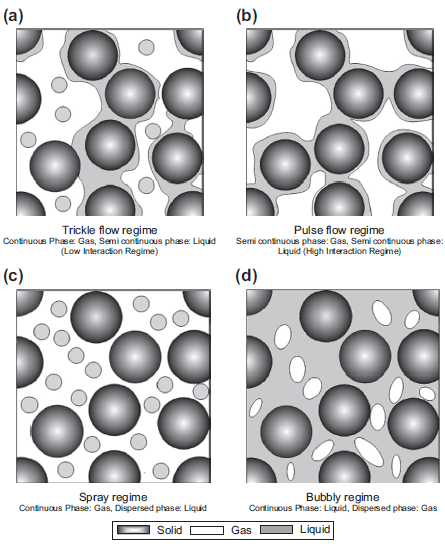
\includegraphics[scale=0.75]{images/Chap2/regimeescoamento.png}
\caption{Regimes de escoamento em reatores de leito gotejante
\cite{Gunjal2005} (extraído de \citeonline{Ranade2011}).}
\label{fig:regimeescoamento}
\end{figure}

O escoamento em regime gotejante ocorre em baixo fluxo de líquido e moderado
fluxo de gás. Como já foi dito, o líquido escoa em forma de filmes ou filetes
sobre as partículas do catalisador. Nesse regime de escoamento, a fase contínua
é a gasosa e a fase líquida escoa dispersa. Esse tipo de escoamento também é
chamado de regime de baixa interação \cite{Saroha1996}.

Em fluxo moderado de líquido e gás ocorre o escoamento em regime pulsante,
caracterizado pelo escoamento semicontínuo de ambas as fases. Ante o regime
por gotejamento, o regime de pulso apresenta maior interação entre as fases.
Todavia, esse processo faz com que regiões ricas em gás se alternem com regiões
ricas em líquido \cite{Saroha1996}.

Os outros dois regimes de escoamento encontrados em TBRs são: borbulhamento e
tipo spray. No primeiro, a fase contínua é a líquida, enquanto que a fase gasosa
escoa dispersa; no segundo, a fase contínua é a gasosa, e a fase líquida é
dispersa. Ambos os casos são classificados como regimes de alta interação entre
as duas fases \cite{Saroha1996}.

Os reatores industriais operam com frequência próximos à transição entre os
regimes gotejante e pulsado. Isso proporciona melhores taxas de transferência de
massa, utilização do catalisador e aumenta a capacidade produtiva
\cite{Ancheyta2011}.

\subsection{Parâmetros Hidrodinâmicos}
\label{sec:parametroshidrodinamicos}

Por natureza, os TBRs possuem uma complexidade fenomenológica ímpar quando se
trata de seu comportamento hidrodinâmico. Superam em complexidade os FBRs,
onde há apenas uma fase escoando pelo leito catalítico. 

A compreensão e a previsão, ainda que imprecisamente, dos parâmetros
hidrodinâmicos dos TBRs são as chaves para o projeto e análise desse tipo de
reator. Os parâmetros sobre os quais serão discorridos a seguir são:

\begin{itemize}
  \item Perda de carga;
  \item Retenção de líquido;
  \item Molhamento das partícutas de catalisador;
  \item Coeficientes de transferência de massa;
  \item Dispersões axial e radial de massa.
%  \item Transferência de calor em TBRs
\end{itemize}

\subsubsection{Perda de Carga}
\label{sec:perdadecarga}

A capacidade de estimar a perda de carga em TBRs na fase de projeto é de suma
importância. Ela definirá a capacidade de um dos equipamentos mais custosos do
sistema, que é o compressor que fará a recirculação da fase gasosa. A perda de
carga também é um importante parâmetro a ser acompanhado pelos engenheiros quando o
TBR está em operação.

A perda de carga bifásica ao longo do reator está relacionada com: (i) a
geometria do reator (diâmetro, tamanho e forma do catalisador e geometria dos
internos, tais como prato distribuidor); (ii) parâmetros operacionais tais como
vazão de gás e líquido (regime de escoamento); e (iii) propriedades das fases
(densidade, viscosidade, tensão superficial etc.). Temperatura e pressão de operação afetam
indiretamente a perda de carga através das propriedades do fluido
\cite{Ranade2011}.

Normalmente as equações de perda de carga são definidas em termos de perda de
carga específica $\Delta P/L$, que é definida como a variação da pressão interna
por unidade de comprimento do reator. Em reatores cujo regime é de baixa
interação (regime gotejante de escoamento), a perda de carga tende a ser
pequena. Para regimes de alta interação, a perda de carga pode chegar a algumas
atmosferas por metro \cite{Benkrid1997}.

\nomenclature[G]{$\Delta P/L$}{Perda de carga por unidade de comprimento de
reator \nomunit{kPa/m}}

Segundo \citeonline{Holub1993}, os modelos hidrodinâmicos podem ser
classificados em duas categorias. A primeira categoria lança mão do empirismo
baseado em análise dimensional para produzir correlações de perda de carga e
retenção de líquido. A segunda categoria utiliza equações do tipo Ergun
\apud{Ergun1952}{Holub1993}, modificando parâmetros para escoamento bifásico.
Essa abordagem é aplicada especialmente para regimes de escoamento de baixa
interação.

\citeonline{Holub1993}, por exemplo, desenvolveram uma correlação para perda
de carga para TBRs operando em regimes de baixa interação. Já
\citeonline{Benkrid1997} utilizaram dados experimentais  da literatura para
propor modelos simples de perda de carga em TBRs que operam em regimes de alta
interação. Ambos os autores citados também desenvolveram
correlações para retenção de líquido.

Diferentemente de muitos autores, que propuseram equações utilizando dados
experimentais coletados em pressões atmosféricas, \citeonline{Larachi1991}
construíram correlações tanto para perda de carga quanto para retenção de
líquido, em pressões de até \SI{8,1}{MPa}.

\subsubsection{Retenção de Líquido}
\label{sec:retencaodeliquido}

A retenção de líquido (\emph{liquid holdup}) em um leito de TBR  pode ser
expressada de duas maneiras: (i) retenção total ($\epsilon^L$), definida como o
volume de líquido por unidade de volume de leito e (ii) saturação de líquido
($\beta_L$), definida como o volume de líquido por unidade de volume vazio (ao
invés de volume total de leito).

A retenção de líquido é composta de duas partes: estática ($\epsilon_{Ls}$) e
dinâmica ($\epsilon_{Ld}$). Por retenção de líquido estática entende-se a
porção de líquido que permanece na superfície das partículas de catalisador após o
leito ser drenado. A fração removida de líquido no processo de drenagem é
definida como retenção dinâmica \cite{Ranade2011}. Alguns autores utilizam como
referência a saturação de líquido estática ($\beta_{Ls}$) e saturação de líquido
dinâmica ($\beta_{Ld}$).

Há algumas ténicas para determinação da retenção de líquido em TBRs. De acordo
com \citeonline{Benkrid1997}, a técnica mais comum é a da drenagem, já
mencionada. Essa técnica consiste em cessar simultaneamente a alimentação de gás
e líquido no reator (topo), coletando o líquido na saída (fundo). O volume de
líquido drenado significará diretamente $\epsilon_{Ld}$. Outra técnica consiste
em determinar a massa do reator enquanto seco e em operação, quando gás e
líquido estarão escoando pelo leito catalítico. Esse método levará diretamente à
determinação de $\beta_L$. \citeonline{Larachi1991} utilizam a distribuição do
tempo de residência para chegar a $\beta_L$.

Vários fatores em TBRs são dependentes da retenção de líquido, tais como fator
de molhabilidade e coeficientes de transferência de massa e calor. A retenção de
líquido também determina o tempo de residência de líquido dentro do reator e,
portanto, a conversão dos reagentes \cite{Ranade2011}.

A consequência das definições apresentadas nessa seção podem ser sumarizadas
da seguinte forma:
\begin{equation}
\epsilon^L + \epsilon^G = \epsilon_B
\label{eq:balancoespaco1}
\end{equation}
sendo $\epsilon_B$ a porosidade do leito e $\epsilon^G$ a retenção de gás.

\nomenclature[G]{$\epsilon^{L}$}{Retenção total de líquido}
\nomenclature[G]{$\epsilon_{Ls}$}{Retenção estática de líquido}
\nomenclature[G]{$\epsilon_{Ld}$}{Retenção dinâmica de líquido}
\nomenclature[G]{$\epsilon_{B}$}{Porosidade do leito}
\nomenclature[G]{$\beta_L$}{Saturação de líquido}
\nomenclature[G]{$\beta_{Ls}$}{Saturação de líquido estática}
\nomenclature[G]{$\beta_{Ld}$}{Saturação de líquido dinâmica}

\subsubsection{Molhamento das Partículas de Catalisador}
\label{sec:molhamento}

Dentre os diversos tipos de reatores multifásicos, o molhamento das partículas
de catalisador é um fenômeno exclusivo em TBR. Levando-se em conta que em um
TBR a fase líquida escoa de forma não uniforme, a determinação do molhamento do
catalisador é uma tarefa bastante difícil \cite{Ranade2011}

Na literatura são definidos dois tipos de molhamento. \citeonline{Colombo1976}
os descrevem assim:

\begin{itemize}
	\item Molhamento interno ou enchimento de poro: é o volume de líquido dentro
	dos poros do catalisador. Como as partículas de catalisador são quase sempre
	porosas, o molhamento interno é considerado total devido ao efeito de
	capilaridade;
	\item Molhamento externo: é a área externa à partícula de catalisador
	efetivamente em contato com o líquido que escoa. Praticamente toda a
	transferência de massa entre o líquido presente nos poros do catalisador e o
	líquido que escoa por sobre as partículas ocorre nessa área.
\end{itemize}

Isto posto, a \emph{eficiência de molhamento} ($\eta_{CE}$) deriva da definição
de molhamento externo. Em outras palavras, ela é definida como sendo a
porcentagem da área superficial externa do catalisador que está efetivamente em
contato com o líquido que escoa \cite{Schwartz1976}.

De acordo com a literatura disponível, a medição da eficiência de molhamento
pode ser direta e indireta. Entre os métodos diretos estão técnicas
fotográficas, método de injeção de corante, imagem de ressonância magnética,
entre outros \apud{Sederman2001}{Ranade2011}. Já os métodos indiretos são
aplicáveis a unidades industriais além de possuirem melhor custo-benefício
\cite{Ranade2011}. \citeonline{Colombo1976} e \citeonline{Schwartz1976}, por
exemplo, utilizaram métodos baseados tanto em taxa de reação quanto em
transferência de massa para determinar a eficiência de molhamento.

\nomenclature[G]{$\eta_{CE}$}{Eficiência de molhamento}

\subsubsection{Coeficientes de Transferência de Massa}
\label{sec:coeficientes}

Em reatores com escoamento gotejante não há um mecanismo severo de mistura como
em outros tipos de escoamento (tanques de mistura ou regimes de alta interação).
Logo, as taxas de transferência de massa são menores em TBRs do que em outros
reatores, podendo limitar a taxa das reações. Os três tipos de taxas de
transferência de massa relevantes nos TBRs são: gás-líquido, líquido-sólido e
gás-sólido \cite{Ranade2011}.

A ocorrência desses tipos de transferência de massa dependerá da eficiência de
molhamento e da retenção de líquido. Em reatores com eficiência de molhamento
próxima à totalidade, por exemplo, desconsidera-se a transferência de massa
gás-sólido \cite{Ranade2011}.

\subsubsection{Dispersões Axial e Radial de Massa}
\label{sec:dispersoes}

As dispersões axial e radial são dois fenômenos que ocorrem em TBRs,
desviando-os da idealidade de escoamento contida no conceito de PFR (PFR -
\emph{Plug-Flow Reactor}).

\nomenclature[Z]{PFR}{Reator de escoamento empistonado}

A dispersão radial está diretamente ligada à distribuição de líquido na entrada
do reator. Esse efeito possui uma quantidade pequena de estudos na literatura. A
razão entre o diâmetro do reator e o diâmetro da partícula de catalisador
($D_R/d_p$) influenciam na relevância da distribuição radial de massa
\cite{Saroha1998}. \citeonline{Al-Dahhan1994}, por exemplo, sugerem que, mesmo
para reatores em alta pressão, um valor de $D_R/d_p > 20$ minimiza o efeito de
má distribuição de líquido em TBR.

Diferente do que ocorre com a dispersão radial, a dispersão axial é um fenômeno
amplamente estudado, com várias referências na literatura. Esse fenômeno está
ligado a retromistura de líquido dentro do leito catalítico e está relacionado
com a razão entre o comprimento do reator e diâmetro da partícula de catalisador
($L_R/d_p$) \cite{Ancheyta2011}. \cite{Mears1971b} propôs um critérios para
verificar se a dispersão axial é relevante ou não, baseando-se no número de
Peclet ($Pe$). O critério de Mears é apresentado da seguinte maneira:

\begin{equation}
\dfrac{L_{R}}{d_p} > \dfrac{20.n}{Bo}ln\left(\dfrac{C_o}{C_f}\right)
\label{eq:Mearscriterio}
\end{equation}

\begin{equation}
Bo = \dfrac{ud_p}{D}
\label{eq:Bodenstein}
\end{equation}

 \begin{equation}
 Pe = \dfrac{uL_{R}}{D}
 \label{eq:Peclet}
 \end{equation}
onde $C_o$ é a concentração do reagente na entrada do reator, $C_f$ é a
concentração do reagente na saída do reator, $L$ é o comprimento do reator, $n$
é a ordem da reação e $Bo$ (número Bodenstein) é o número de $Pe$ baseado no
diâmetro da partícula.

\nomenclature{$D_{R}$}{Diâmetro do reator \nomunit{m}}
\nomenclature{$L_{R}$}{Comprimento total do reator \nomunit{m}}
\nomenclature{$d_{p}$}{Diâmetro da partícula de catalisador \nomunit{m}}
\nomenclature{$Bo$}{Número de Bodenstein}

Alguns fatores que contribuem na distribuição de líquido e na retromistura são:
capilaridade, existência de zonas-mortas, molhamento parcial e caminhos
preferenciais \cite{Ranade2011}.

\subsection{Reações Químicas em TBR} \label{sec:reacoestbr}
 
As reações químicas em TBRs possuem uma complexidade maior ante as reações
homogêneas justamente pela presença de um catalisador sólido. A superfície
de uma partícula de catalisador, em toda a sua complexidade, apresenta-se
como o local onde as reações ocorrem. Além disso, fenômenos de transporte
de massa podem influenciar na taxa global da reação \cite{Froment2011}. 

Sendo assim, os passos envolvidos em uma reação química, na superfície de um
catalisador, para um reator cujo escoamento é monofásico são \cite{Froment2011}: 

\begin{enumerate}
\item Transporte dos reagentes do seio do fluido para a superfície
do catalisador;
\item Transporte dos reagentes nos poros do catalisador;
\item Adsorção dos reagentes no sítio catalítico;
\item Reação química entre os átomos ou moléculas;
\item Dessorção dos produtos;
\item Transporte dos produtos da reação dos poros de volta à
superfície do catalisador;
\item Transporte dos produtos da superfície das partículas para o seio do
fluido.
\end{enumerate} 

Segundo \apudonline{Ramachandran1983}{Ranade2011}, para os TBRs onde as
partículas de catalisador estão completamente molhadas (velocidade superficial
de líquido \SI{>0,5}{\centi\meter\per\s}), os passos apontados por
\citeonline{Froment2011} ganham novas etapas, como segue:

\begin{enumerate}
\item Transporte dos reagentes presentes na fase gasosa para o seio da
fase líquida;
\item Transporte dos reagentes presentes na fase líquida para a superfície do
catalisador;
\item Transporte dos reagentes nos poros do catalisador;
\item Adsorção dos reagentes no sítio catalítico;
\item Reação química entre os átomos ou moléculas;
\item Dessorção dos produtos;
\item Transporte dos produtos da reação dos poros de volta à superfície do
catalisador;
\item Transporte dos produtos da superfície das partículas para o seio da fase
líquida;
\end{enumerate} 

Pode haver ainda mais um passo em que um dos produtos, se termodinamicamente
favorável, passasse para a fase gasosa. Em reatores de hidrotratamento de
diesel, por exemplo, o \ce{H2S} produzido descola-se parcialmente para a fase
gasosa, diminuindo a pressão parcial de hidrogênio. O hidrogênio nesse caso é
o reagente em excesso \cite{Ancheyta2011}.

Entretanto, muitos TBRs comerciais operam com velocidades superficiais de
líquido baixas \SI{<0,5}{\centi\meter\per\s}. Isso faz com que o regime de
escoamento seja classificado como de baixa interação e, consequentemente, não molha
completamente a superfície das partículas. Nesse caso, a taxa de reação
dependerá da fase em que está o reagente limitante \cite{Ranade2011}.

\section {Modelagem de Reatores de Leito Fixo} \label{sec:modelagemreatores}

Várias formas de modelagem de FBRs podem ser encontradas na literatura.
Segundo \citeonline{Froment2011}, os modelos podem ser categorizados em dois
grandes grupos: pseudo-homogêneos e heterogêneos. Por modelos
pseudo-homogêneos entende-se aqueles que não fazem distinção entre as fases,
i.e., não considera a presença do catalisador. Em se tratando de um TBR, não há
também distinção entre as fases líquida e gasosa. Já modelos heterogêneos
distinguem, no mínimo, duas fases concomitantes.

Ainda de acordo com \citeonline{Froment2011}, os FBR podem ser classificados em
unidimensionais e bidimensionais. Os modelos bidimensionais consideram
gradientes radiais de massa e/ou calor. Já modelos unidimensionais consideram a
idealidade de escoamento empistonado, podendo ou não contemplar a dispersão
axial.

Modelos matemáticos também podem ser categorizados ou como de
descrições empíricas (também chamados de modelos caixa-preta) ou que se baseiam
em primeiros princípios. Como nome diz, modelos de primeiros princípios
utilizam-se das leis químicas e físicas (balanço de massa e energia,
termodinâmica, cinética das reações). Por outro lado, modelos empíricos são
utilizados quando há falta de tempo e/ou informações para o
desenvolvimento de modelos de primeiros princípios. Nesses modelos, são
necessárias informações de entrada e saída para ajustar coefientes nas equações
que os compõem \cite{Edgar2001}.

De forma genérica, \citeonline{Rasmuson2014} classificam modelos matemáticos
em pares opostos, por exemplo: determinísticos versus estocásticos; contínuos
versus discretos. 

De acordo com \citeonline{Rasmuson2014}, os modelos determinísticos são aqueles
em que a cada variável e parâmetro pode ser atribuído um número fixo definido,
ou uma série de números, para um dado conjunto de condições, i.e., o modelo não
possui componentes que sejam incertos. Em contraste, a incerteza é
introduzida nos modelos estocásticos. Neste tipo de modelo, 
as variáveis ou parâmetros utilizados para descrever as relações de
entrada-saída não são precisamente conhecidas. Além disso, Um modelo estocástico
envolve parâmetros caracterizadas por distribuições de probabilidade. Por essa
razão, tais modelos podem apresentar diferentes resultados em cada simulação.

Segundo \citeonline{Rasmuson2014}, em modelos contínuos as variáveis
podem assumir qualquer valor dentro de um intervalo definido. Em se tratando de
PBR, \citeonline{Ancheyta2011} modelos contínuos contêm um conjunto de equações
diferenciais com uma ou mais variáveis independentes, onde todas devem ser
resolvidas simultaneamente. Em contrapartida, modelos discretos consideram que as
variáveis assumem apenas um valor dentro de um determinado intervalo
\cite{Rasmuson2014}. Diferentemente dos modelos contínuos (equações
diferenciais), a modelagem discreta encarrega-se de resolver equações algébricas
para o caso de estado estacionário, ou equações diferenciais ordinárias quando
se trata de simulação dinâmica \cite{Schnitzlein1987}.

\citeonline{Deans1960} são apontados como os primeiros a construir um modelo
baseado em estágios discretos em TBRs, chamado de \emph{rede de células} por
alguns autores (\citeonline{Schnitzlein1987} e \citeonline{Ancheyta2011}, por
exemplo). \citeonline{Deans1960} utilizaram o método de modelagem por rede
de células para estudar os fenômenos de dispersão axial e radial em um TBR.
Segundo \citeonline{Schnitzlein1987}, independente do arranjo das células, a
descrição do sistema reacional dentro de cada célula pode ser pseudo-homogêneo ou
heterogêneo.

Outra abordagem de modelagem discreta são os modelos \emph{baseados em
estágios}. Nesses modelos utiliza-se \emph{abordagem baseada em taxa}, que é
fundamentada na aplicação direta dos fenômenos de difusão, transferência de
calor e dos efeitos de interação multicomponente no cálculo de cada segmento
(estágio). Essa abordagem é bastante utilizada em processos de separação tais
como destilação e extração \cite{Jakobsson2004}. Foi com essa abordagem que
\citeonline{Jakobsson2004} modelaram reatores de hidrotratamento de diesel, em
suas operações contracorrente e cocorrente.

\section {Modelagem e Simulação de Hidrogenação Seletiva de Gasolina de Pirólise}
\label{sec:hidrogenacaopygas}

O primeiro estágio de hidrogenação da gasolina de pirólise, também conhecido
como hidrogenação seletiva, foi estudado por alguns autores encontrados na
literatura, incluindo algumas avaliações de resposta dinâmica. A seguir serão
apresentados alguns estudos publicados.

\subsection{Descrição Geral do Processo} \label{sec:descricaogeral}

Tipicamente, a gasolina de pirólise é hidrogenada em um reator tipo TBR, onde o
catalisador pode ser de paládio ou níquel suportado em alumina. Normalmente, o
reator possui ao menos dois leitos. Devido à exotermicidade das reações, há uma
injeção de \emph{quench} líquido entre os leitos, composta de produto
hidrogenado resfriado, que serve para controlar a temperatura do segundo leito e
evitar o coqueamento sobre a superfície do catalisador. O produto hidrogenado
pode também diluir a carga do reator, retardando o processo de desativação já
mencionado \cite{Cheng1986,Derrien1986,Arpornwichanop2002,Rojas2014a}.

\subsection{Cinética das Reações} \label{sec:cinetica}

As duas principais reações que ocorrem em reatores de hidrogenação de gasolina
de pirólise são a conversão de diolefinas em olefinas e de olefinas em
parafinas, que ocorrem de forma sequencial. Como já mencionado, o grau de
hidrogenação dependerá da utilização final da corrente hidrogenada
\cite{Cheng1986}.

\citeonline{Cheng1986} publicaram valores de constantes cinéticas para a
hidrogenação de gasolina de pirólise, agrupando os compostos em diolefinas,
olefinas e parafinas. Além disso, as reações foram tratadas como irreversíveis,
da seguinte forma:
\begin{equation}
\textrm{Diolefinas} \rightarrow \textrm{Olefinas} \rightarrow \textrm{Parafinas}
\label{eq:hidrogenacao}
\end{equation}

Enfim, \citeonline{Cheng1986} estimaram as constantes cinéticas assumindo que
as reações fossem de pseudo-primeira ordem, ou seja, a concentração de
hidrogênio na fase líquida foi assumida como constante.

\citeonline{Authayanun2008} apresentam uma simulação de um reator de
hidrogenação parcial de gasolina de pirólise. Um dos objetivos deste trabalho
foi a determinação das constantes de velocidade específicas, assumindo as
mesmas considerações feitas por \citeonline{Cheng1986}, exceto que as
reações fossem de pseudo-primeira ordem, \emph{i.e.}, a concentração de
hidrogênio compôs a equação da velocidade das reações. Além disso, foi
adicionado um termo de adsorção à cinética de reação das olefinas, uma vez que a
reação destas é fortemente influenciada pela concentração de diolefinas, como
demonstrado recentemente por \citeonline{Zhou2010}.

\citeonline{Rojas2014a} e \citeonline{Mostoufi2005a} utilizaram praticamente as
mesmas premissas apresentadas por \citeonline{Cheng1986}, porém com uma
diferença: os compostos insaturados não foram agrupados em diolefinas
(pentadieno e ciclopentadieno, por exemplo) ou olefinas (penteno e
ciclopenteno). As cinéticas foram específicas para cada composto reagente.
\citeonline{Hanika1999} apresentam as reações e os parâmetros cinéticos
utilizados por \citeonline{Rojas2014a} e \citeonline{Mostoufi2005a}.

\subsection{Considerações sobre Propriedades Físicas e Equilíbrio Líquido-Vapor}
\label{sec:consideracoeselv}

Como já mencionado na \autoref{sec:modelagemreatores}, modelos de reatores
determinísticos contínuos necessitam resolver um sistema de equações
diferenciais para obter os resultados de simulação. Nesses modelos, a inserção
de equações que descrevam o equilíbrio líquido-vapor (ELV) é trabalhoso. Em
TBRs de hidrotratamento de diesel, segundo \citeonline{Ancheyta2011}, as
premissas de (i) fase gasosa em excesso, cuja composição é próxima a de
hidrogênio puro, e (ii) de que os compostos em fase líquida não mudam de fase,
facilitam os cálculos por essa abordagem.

Nos estudos realizados por \citeonline{Authayanun2008},
\citeonline{Arpornwichanop2002}, \citeonline{Arpornwichanop2008} e
\citeonline{Mostoufi2005a} as propriedades das fases gasosa e líquida foram
mantidas constantes ao longo de todo o reator, inclusive a concentração de
hidrogênio na fase líquida. A consequência disso é que, nesses trabalhos, os
efeitos de aquecimento tanto na taxa da reação quanto nos fenômenos
hidrodinâmicos permanecem desconhecidos.

Entretanto, \citeonline{Rojas2014a}, em sua modelagem de um reator de
gasolina de pirólise, modelam o ELV através de um \emph{flash} adiabático,
utilizando a abordagem $\phi-\phi$, onde uma equação de estado é utilizada para
o cálculo de equilíbrio de fases. Isso foi feito porque um dos objetivos do
trabalho foi comparar diferentes equações de estado (e seus parâmetros) quanto a
solubilidade de hidrogênio em gasolina de pirólise; a base termodinâmica
utilizada está no trabalho de \citeonline{Rojas2014}, que é uma extensão do
estudo feito por \citeonline{Zhou2006}.
\nomenclature[Z]{ELV}{Equilíbrio Líquido-Vapor}

\subsection{Hidrodinâmica} \label{sec:hidrodinamica}
Todos os trabalhos encontrados sobre hidrogenação parcial de gasolina de
pirólise classificam o reator como um TBR \cite{Arpornwichanop2002,
Authayanun2008, Mostoufi2005a, Arpornwichanop2008, Rojas2014a}. 

O trabalho de \citeonline{Rojas2014a} destaca-se dos demais autores
citados por considerar o regime de escoamento do reator como sendo do tipo
borbulhamento, ainda que ambas as fases estejam em escoamento descendente.
Assim, algumas equações hidrodinâmicas consideradas são diferentes das
utilizadas pelos demais trabalhos.

\subsection{Transferência de Massa} \label{sec:transferenciamassa}

Sobre o fenômeno de transferência de massa do sistema difusão-reação, 
os autores adotaram posturas conforme as respectivas abordagens cinéticas.

Assim, o grupo de autores que agrupou os compostos em diolefinas, olefinas e
parafinas \cite{Arpornwichanop2002, Authayanun2008} e, ainda, que considerou o
hidrogênio na cinética da reação, também tratou da difusão deste composto da
fase gasosa até a superfície do catalisador. 

Em contrapartida, \citeonline{Rojas2014a} e \citeonline{Mostoufi2005a}, por
terem utilizado como base o trabalho de \citeonline{Hanika1999} para a cinética
das reações, consideraram a fase gasosa em grande excesso e, portanto,
neglicenciaram a resistência à transferência de massa na fase gasosa.
Logo, segundo esses autores, a resistência à transferência de massa
mais influente está na fase líquida (interface líquido-sólido).

\subsection{Abordagens de Modelagem} \label{sec:abordagensmodelagem}

Os pesquisadores que publicaram trabalhos sobre hidrogenação de gasolina
de pirólise, seja a hidrogenação parcial, seja a hidrogenação total, modelaram
os reatores utilizando modelos determinísticos contínuos. A diferença entre
eles fica a cargo do método númerico aplicado. Vale destacar que no caso de
\citeonline{Rojas2014a}, foi elaborado um algoritmo para a resolução
do reator, e que ainda utilizou de simulador comercial para o cálculo de ELV.

Não foi encontrado qualquer artigo que utilizasse a modelagem por rede de
células para o processo de hidrogenação de gasolina de pirólise.

%\section{Considerações Finais} \label{sec:consideracoesfinais}

%
\chapter{Metodologia}
\label{chap:metodologia}

\section{Descrição do Processo} \label{sec:descricaoprocesso}

Como já mencionado no \autoref{chap:introducao}, o processo modelado
neste trabalho utilizou os dados publicados por \citeonline{Rojas2014a}. 

\subsection{Diagrama Esquemático} \label{sec:diagramaesquematico}

O reator é composto de dois leitos catalíticos, carregados de forma densa
(\emph{dense loading}). No topo de ambos os leitos há catalisador carregado de
forma solta (\emph{sock loading}). A carga é composta de gasolina de pirólise,
hidrogênio e parte do produto hidrogenado reciclado. Este último é parte da
corrente líquida oriunda de um vaso de separação, cuja carga é a corrente de
saída do reator. Parte da corrente líquida do vaso de separação também
funciona como corrente de resfriamento, que é injetada entre os dois leitos
catalíticos para controle de temperatura (\emph{quench}). Um diagrama
simplificado que ilustra o reator está na \autoref{fig:esquemareator}. 

\begin{figure}[htb]
\centering 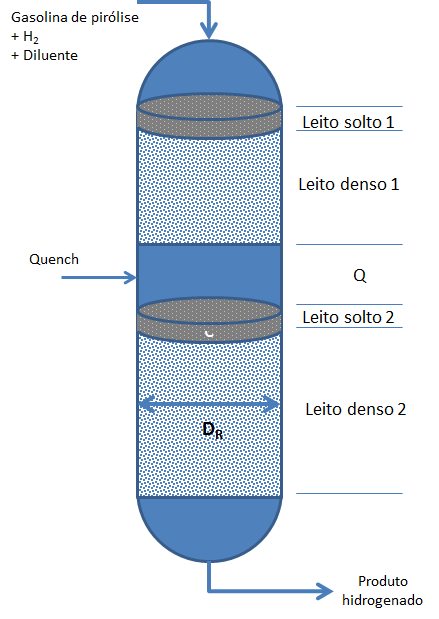
\includegraphics[scale=0.75]{images/Chap3/esquemareator.png}
\caption{Diagrama esquemático do reator \cite{Rojas2014a}.}
\label{fig:esquemareator}
\end{figure}

A \autoref{tab:dadosreator} apresenta as dimensões do reator.

\begin{table}[!htb]
\begin{center}
\caption{Dados do Reator \cite{Rojas2014a}.}
\label{tab:dadosreator}
\small
\begin{tabular}{lcc}
{Dimensão} & {Variável} & {Valor}
\\
\hline
{Diâmetro do Reator} & {$D_R$} & $3,047$ m \\
{Comprimento do Leito Solto 1} & {$L_{sl1}$} & $0,13$ m \\
{Comprimento do Leito Denso 1} & {$L_{dl1}$} & $2,97$ m \\
{Comprimento do Leito Solto 2} & {$L_{sl2}$} & $0,38$ m \\
{Comprimento Leito Denso 2} & {$L_{dl2}$} & $2,97$ m \\
{Zona de Quench} & {$L_{Q}$} & $1,55$ m \\
\bottomrule
\end{tabular}
\end{center}
\end{table}

\nomenclature{$L_{sl1}$}{Comprimento do leito solto 1 \nomunit{m}}
\nomenclature{$L_{dl1}$}{Comprimento do leito denso 1 \nomunit{m}}
\nomenclature{$L_{sl2}$}{Comprimento do leito solto 2 \nomunit{m}}
\nomenclature{$L_{dl2}$}{Comprimento do leito denso 2 \nomunit{m}}
\nomenclature{$L_{Q}$}{Comprimento da zona de quench \nomunit{m}}

\subsection{Catalisador} \label{sec:catalisador}

O catalisador considerado na modelagem contém Pd suportado em alumina
($Al_2O_3$), de formato esférico. Além desses dados, foi fornecida a informação
de volume total de poros $Vt_{poros}$ = $5,5.10^{-4}$ $m^3/kg$. O dado de volume
total de poros não é suficiente por si só para calcular a porosidade dos leitos,
como é apresentado na \autoref{sec:propriedadesleitoscataliticos}. Assim,
adotou-se a massa específica do $Al_2O_3$ puro ($\rho_{Al_2O_3}$ = $3940$
$kg/m^3$) para a massa específica da parte sólida das partículas de catalisador.

\nomenclature{$Vt_{poros}$}{Volume total de poros \nomunit{m^3/kg}}
\nomenclature[G]{$\rho_{Al_2O_3}$}{Massa específica do óxido de alumínio
\nomunit{kg/m^3}}

\subsection{Porosidade dos Leitos Catalíticos}
\label{sec:propriedadesleitoscataliticos}

Antes de determinar a porosidade dos leitos catalíticos, é preciso avaliar a
massa específica das partículas ($\rho_{p}$). Este parâmetro, calculado pela
\autoref{eq:rhoparticula}, é estimado em $1244 kg/m^3$.

\begin{equation}
\rho_{p} = \dfrac{1}{Vt_{poros}+\dfrac{1}{\rho_{Al_2O_3}}}
\label{eq:rhoparticula}
\end{equation}

\nomenclature[G]{$\rho_{p}$}{Massa específica da partícula de catalisador
\nomunit{kg/m^3}}

A porosidade de cada um dos leitos pode ser calculada, portanto, pela
\autoref{eq:porosidade}, como segue:

\begin{equation}
\epsilon_{B} = \dfrac{V_{l}-\dfrac{\rho_{B}V_l}{\rho_{Al_2O_3}}}{V_l}
\label{eq:porosidade}
\end{equation}

sendo $V_l$ o volume do leito e $\rho_B$ a
massa específica de um leito catalítico logo após o seu carregamento. 

Utilizando os dados apresentados na \autoref{sec:catalisador}, e utilizando os
valores de massa específica \emph{bulk} dos leitos $\rho_{B}$ publicados por
\citeonline{Rojas2014a}, chega-se nos valores mostrados na
\autoref{tab:dadosdosleitos}.

\begin{table}[!htb]
\begin{center}
\caption{Dados dos Leitos Catalíticos \cite{Rojas2014a}.}
\label{tab:dadosdosleitos}
\small
\begin{tabular}{ccc}
{ - } & {Densidade \emph{bulk} ($kg/m^3$)} & {Porosidade} 
\\
\hline
{Leito 1} & $814$ & $0,346$ \\
{Leito 2} & $813$ & $0,347$ \\
\bottomrule
\end{tabular}
\end{center}
\end{table}

Visto que o topo dos leitos, carregados de maneira solta, não são partes
significativas dos leitos, a porosidade destas seções foi
considerada a mesma de carregamento denso para fins de simplificação. 

\subsection{Composição das Correntes} \label{sec:composicaocorrentes}

A composição das correntes de entrada e de quench estão na
\autoref{tab:composicao}. Para o presente trabalho, utilizou-se
apenas os valores da primeira corrida publicados por
\citeonline{Rojas2014a}, já que para este caso foram publicados
também dados industriais.

As propriedades termodinâmicas dos compostos $28$ e $29$ não foram
encontradas. Assim, eles foram considerados como sendo parte dos compostos
$26$ e $27$, respectivamente.

\begin{table}[!htb]
\begin{center}
\caption{Composição das correntes de entrada e de quench \cite{Rojas2014a}.}
\label{tab:composicao}
\small
\begin{tabular}{clcc}
{Identificador $i$} & {Composto} & Entrada (\% mássica) & Quench (\% mássica)
\\
\hline
1 & Hidrogênio				& $0,48$ & $0,08$ \\
2 & Metano					& $0,52$ & $0,70$ \\
3 & Etano					& $0,12$ & $0,11$ \\
4 & n-Propano				& $0,36$ & $0,27$ \\
5 & n-Butano				& $0,30$ & $0,24$ \\
6 & n-Pentano				& $5,40$ & $5,60$ \\
7 & trans-2-Penteno			& $5,30$ & $7,60$\\
8 & trans-1,3-Pentadieno	& $2,50$ & $0,23$ \\
9 & Ciclopentano			& $1,50$ & $2,60$ \\
10& Ciclopenteno			& $2,10$ & $3,00$ \\
11& Metil-1,3-Ciclopentadieno	& $1,90$ & $0,21$ \\
12& n-Hexano				& $3,30$ & $3,30$ \\
13& Metilciclopentano		& $1,60$ & $1,70$ \\
14& Metilciclopenteno		& $2,00$ & $2,60$ \\
15& 1,3-Ciclopentadieno		& $1,90$ & $0,02$ \\
16& Benzeno					& $28,90$ & $30,10$ \\
17& n-Heptano				& $2,80$ & $2,90$ \\
18& Tolueno					& $16,00$ & $16,30$ \\
19& n-Octano				& $1,30$ & $1,30$ \\
20& Etilbenzeno				& $3,40$ & $5,40$ \\
21& Estireno				& $2,00$ & $0,11$ \\
22& Xileno					& $5,40$ & $5,50$ \\
23& n-Nonano				& $0,66$ & $0,72$ \\
24& 1-Metil-3-Etilbenzeno	& $2,90$ & $3,90$ \\
25& Metilestireno			& $1,40$ & $0,31$ \\
26& Dihidrodiciclopentadieno	& $1,80$ & $3,00$ \\
27& Diciclopentadieno		& $1,80$ & $0,12$ \\
28& Metildihidrodiciclopentadieno	& $1,50$ & $2,20$ \\
29& Metildiciclopentadieno	& $0,88$ & $0,11$ \\
\bottomrule
\end{tabular}
\end{center}
Onde $i$ é o número identificador do composto na simulação a ser apresentada.
\end{table}

\nomenclature[S]{$i$}{i-ésimo componente}

\subsection{Condições de operação} \label{sec:condicaocomposicaocorrentes}

As condições de operação consideradas inicialmente estão na
\autoref{tab:condicoesoperacao}. No \autoref{chap:resultados} há uma discussão
sobre a validade de algumas dessas variáveis aqui apresentadas.

\begin{table}[!htb]
\begin{center}
\caption{Dados do Reator \cite{Rojas2014a}.}
\label{tab:condicoesoperacao}
\small
\begin{tabular}{lcc}
{Dimensão} & {Variável Discretizada} & {Valor}
\\
\hline
{Pressão de entrada} & {$P_{1}$} & $5,03$ MPa \\
{Temperatura de entrada} & {$T_{1}$} & $366,15$ K \\
{Vazão mássica de entrada} & {$F_{w,1}$} & $2,477.10^5$ kg/h \\
{Pressão da corrente de \emph{quench}} & {$P_{Q}$} & $4.6$ MPa \\
{Temperatura da corrente de \emph{quench}} & {$T_{Q}$} & $326,15$ K \\
{Vazão mássica da corrente de quench} & {$F_{w,Q}$} & $2,079.10^4$ kg/h \\
\bottomrule
\end{tabular}
\end{center}
\end{table}

\section{Premissas} \label{sec:premissas}

\subsection{Premissas adotadas por \citeonline{Rojas2014a}}
\label{sec:premissasrojas}

Antes de apresentar as premissas que nortearam o presente trabalho, vale
aqui apresentar, para efeito de comparação, as premissas utilizadas por
\citeonline{Rojas2014a}.

\begin{enumerate}
  \item O reator opera em estado estacionário e adiabaticamente.
  \item Gradientes radiais são desprezíveis.
  \item Dispersões axiais foram negligenciadas; portanto, assumiu-se o
  escoamento empistonado para ambas as fases líquida e gasosa.
  \item A fase gasosa está em excesso; dessa forma, negligenciou-se a
  resistência a transferência de massa na fase gasosa.
  \item Fator de molhamento, atividade catalítica e densidade do leito
  uniformes.
  \item A transferência de calor entre as fases e no interior das partículas de
  catalisador foram desprezadas.
  \item A entalpia de dissolução de compostos na fase gás, bem como calor de
  vaposização de líquido foram desprezadas.
  \item A região do quench é assumida como sendo um tambor \emph{flash}, que atinge o
  equilíbrio instantaneamente.
  \item A corrente de saída do primeiro leito mistura-se instantaneamente com a
  corrente de quench.
  \item O reator opera em regime de borbulhamento.
  \item Reações reversíveis e isomerizações foram negligenciadas.
  \item As reações ocorrem somente na interface líquido-sólido.
  \item A desativação catalítica foi desprezada.
\end{enumerate}

No presente estudo, algumas premissas adotadas por \citeonline{Rojas2014a} serão
alteradas, como será descrito a seguir. 

\subsection{Premissas deste trabalho} \label{sec:premissasdestetrabalho}

Como já mencionado no \autoref{chap:introducao}, um dos objetivos do presente
trabalho é avaliar algumas respostas dinâmicas ao processo proposto. Além disso,
a implementação da modelagem foi feita em \emso, software que avalia respostas
dinâmicas por concepção. Assim, convenientemente, a premissa de um reator
operando em estado estacionário foi descartada. Permanece, porém, aqui, a
premissa de que o equipamento opere de forma adiabática.

A alteração mais importante às premissas adotadas por \citeonline{Rojas2014a}, e
que representa um avaço por eles publicado, é a consideração tanto da entalpia
de dissolução do hidrogênio na fase líquida quanto da entalpida de vaporização
de líquido. Isso foi possível graças à abordagem de modelagem por células,
assunto da seção \autoref{sec:modelagemredecelulas}.

Portanto, ficam aqui definidas as seguintes premissas:

\begin{enumerate}
  \item O reator opera adiabaticamente.
  \item Gradientes radiais são desprezíveis.
  \item Dispersões axiais foram negligenciadas; portanto, assumiu-se o
  escoamento empistonado para ambas as fases líquida e gasosa.
  \item A fase gasosa está em excesso; dessa forma, negligenciou-se a
  resistência a transferência de massa na fase gasosa.
  \item Fator de molhamento, atividade catalítica e densidade do leito
  uniformes.
  \item A transferência de calor entre as fases e no interior das partículas de
  catalisador foram desprezadas.
  \item A região do \emph{quench} é assumida como sendo um tambor \emph{flash}, que
  atinge o equilíbrio instantaneamente.
  \item A corrente de saída do primeiro leito mistura-se instantaneamente com a
  corrente de \emph{quench}.
  \item O reator opera em regime de borbulhamento.
  \item Reações reversíveis e isomerizações foram negligenciadas.
  \item As reações ocorrem somente na interface líquido-sólido.
  \item A desativação catalítica foi desprezada.
\end{enumerate}

Um dos motivos de se manter praticamente inalteradas as premissas adotadas por
\citeonline{Rojas2014a} foi o de realiar comparações entre os dois estudos.

Negligenciar os gradientes e dispersões de calor e massa, tanto radialmente
quanto axialmente, é uma recomendação muito comum encontrada na literatura
\cite{Ancheyta2011, Ranade2011, Froment2011} para simulações cujo objetivo é
prever o comportamento de um TBR, sob o ponto de vista de liberação de calor e
conversão das reações. Da mesma forma é a desconsideração da transferência de
calor entre as fases.

Como já mencionado no \autoref{chap:revisaobibliografica},
\citeonline{Rojas2014a} utilizaram as reações publicadas por
\citeonline{Hanika1999}. Isso pode ter motivado os autores a negligenciar a
resistencia à transferência de massa na fase gasosa.

As premissas assumidas para a região de \emph{quench} são bastante razoáveis, já
que normalmente os projetistas de reatores TBR desejam a corrente oriunda do
leito superior se misture rapidamente com a corrente de \emph{quench},
homogeneizando a carga para o segundo leito. Uma mistura inadequada entre as
correntes de entrada na região de \emph{quench} pode levar a caminhos
preferenciais e regiões de estagnação no leito inferior \cite{Ancheyta2011}.

O regime de operação por borbulhamento foi adotado para que as
equações hidrodinâmicas fossem as mesmas utilizadas por \citeonline{Rojas2014a}.
Contudo, uma verificação da validade dessa premissa é apresentada no
\autoref{chap:resultados}.

\section{Modelagem por Rede de Células} \label{sec:modelagemredecelulas}

Para utilizar a abordagem de modelagem por rede de células, cada leito
catalítico foi subdivido em células em seu comprimento, i.e., discretizado em
$N_{Disc}$ segumentos de leito. Cada seguimento de leito fica identificado por
um índice ($z$). A figura \autoref{fig:celula} ilustra uma célula de leito de
reator. Do ponto de vista reacional, cada célula representará um reator CSTR
associado a um tambor de \emph{flash}. Nesse tambor de \emph{flash}, mantém-se a premissa
de que o equilíbrio termodinâmico é atingido instantaneamente.

 \begin{figure}[htb]
 \centering 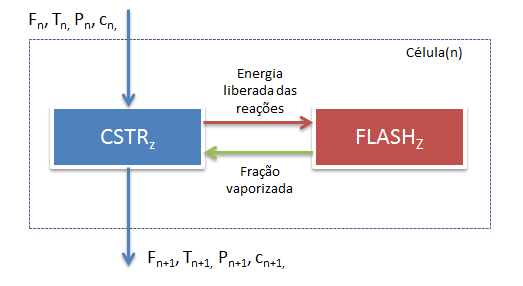
\includegraphics[scale=0.75]{images/Chap3/celula.png}
 \caption{Elemento discretizado de leito - célula}
 \label{fig:celula}
 \end{figure}

\nomenclature{$N_{Disc}$}{Número de células de um leito do reator}
\nomenclature[S]{$z$}{z-ésima célula de leito de reator}

Para a região de quench, será usado um tambor de \emph{flash}, onde o equilíbrio
termodinâmico é também atingido instantaneamente. A \autoref{fig:quench} ilustra
a região de quench.

 \begin{figure}[htb]
 \centering 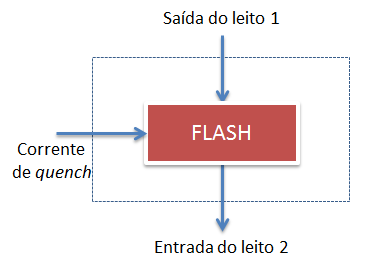
\includegraphics[scale=0.75]{images/Chap3/quench.png}
 \caption{Região de quench do reator}
 \label{fig:quench}
 \end{figure}

Com esse tipo de abordagem, foi possível considerar os efeitos termodinâmicos
ao longo do reator, como também prever a composição das fases líquida e
gasosa. As próximas seções apresentam o equacionamento construído

\section{Balanço de Massa e Energia} \label{sec:balancomassaenergia}

Normalmente, para a modelagem de TBR heterogênea, os autores que utilizam
modelos determinísticos contínuos fazem o balanço de massa para todas as
fases separadamente, i.e., para cada fase é feito o balanço de massa por
componente. %\citeonline{Ancheyta2011} apresenta de uma forma didática as
% equações de balanço de massa de cada fase, considerando e explicando todos os
% efeitos (dispersões, reações, transferências de massa).
Cada pesquisador, portanto, de acordo com a premissa adotada, elimina muitos dos
termos das equações de balanço, a fim simplificar o modelo e facilitar a
solução. 

Para este trabalho, diante das premissas adotadas, a equação de balanço de massa
está mostrada na \autoref{eq:balancodemassa}. Nessa equação, foi considerado o
termo de diferenciação da massa $M$ de cada componente $i$, em cada célula $z$,
no tempo $t$. Dessa forma, é possível o estudo de respostas dinâmicas do
processo.

\begin{equation}
\dfrac{dM_{i,z}}{dt} = F_zC_{i,z} - F_{z+1}C_{i,z+1} +
\displaystyle\sum_{j=1}^{N_{reac}} \nu_{i,j}r_{j,z} \dfrac{W}{N_{Disc}}
\label{eq:balancodemassa}
\end{equation}

onde $M_{i,z}$ é a massa do componente $i$ na célula $z$, $j$ é o número
identificador de cada reação, $N_{reac}$ é o número total de reações,
$\nu_{i,j}$ é o coeficiente do componente $i$ na reação $j$, $r_{j,z}$ é taxa
da reação $j$ na célula $z$, $F$ é a vazão molar total e $W$ é a massa total de
catalisador presente no leito.

\nomenclature{$M$}{Massa \nomunit{kmol}}
\nomenclature{$N_{reac}$}{Número total de reações}
\nomenclature{$r$}{Taxa de reação \nomunit{kmol/(kg_{cat}.h)}}
\nomenclature{$F$}{Vazão molar \nomunit{kmol/h}}
\nomenclature{$W$}{Massa total de catalisador em um leito\nomunit{kg}}
\nomenclature[S]{$j$}{j-ésima reação}
\nomenclature[G]{$\nu$}{Coeficiente de reação}

A \autoref{eq:balancodeenergia} mostra o balanço de energia de forma
discretizada.

\begin{equation}
\dfrac{dE_{z}}{dt} = F_zh_{z} - F_{z+1}h_{z+1} +
\displaystyle\sum_{j=1}^{N_{reac}} \Delta H_{j}r_{j,z} \dfrac{W}{N_{Disc}}
\label{eq:balancodeenergia}
\end{equation}

onde $E_{z}$ é a energia na célula $z$,  $h$ é a entalpia da
corrente $F$ e $\Delta H_{j}$ o calor envolvido na reação $j$.

\nomenclature{$E$}{Energia \nomunit{kJ}}
\nomenclature{$h$}{Entalpia \nomunit{kJ/kmol}}
\nomenclature[G]{$\Delta H$}{Calor de reação \nomunit{kJ/kmol}}

As \autoref{eq:balancodemassa} e \autoref{eq:balancodeenergia}, somadas a
corrente $F$ e seu cálculo de ELV, permitem determinar a fração vaporizada,
composição das fases e respectivas propriedades físicas em cada célula $z$.

É importante notar ainda que, da forma como as \autoref{eq:balancodemassa} e
\autoref{eq:balancodeenergia} estão escritas, massa e energia contidas em cada
célula são grandezas extensivas. 

\section{Cinética das Reações} \label{sec:cineticadasreacoes}

As reações de hidrogenação e os parâmetros cinéticos estão na
\autoref{tab:composicao}. Conforme já explicado, o sistema reacional foi
considerado como sendo um conjunto de hidrogenações irreversíveis e
independentes da concentração de hidrogênio. A constante de pseudo-primeira
ordem da reação $j$ na célula $z$, $k^{'}_{j,z}$, está definido na
\autoref{eq:constantepseudoprimeiraordem}.

\begin{equation}
k^{'}_{j,z} = \eta_ik_jC^{*}_{H_2}
\label{eq:constantepseudoprimeiraordem}
\end{equation}

sendo $\eta$ o fator de efetividade de intradifusão, $k$ a
constante de taxa de reação instrínseca e $C^{*}_{H_2}$ a concentração de
equilíbrio de hidrogênio em fase líquida.

\nomenclature{$k^{'}$}{Constante de taxa de reação de pseudo-primeira
ordem \nomunit{kg/(kg_{cat}.h)}}
\nomenclature{$k$}{Constante de taxa de reação intrínseca
\nomunit{kg.m^3/(kg_{cat}.h.kmol_{H_2})}}
\nomenclature{$C^{*}_{H_2}$}{Concentração de equilíbrio de hidrogênio em fase
líquida \nomunit{kmol/m^3} \nomunit{kJ/kmol}}
\nomenclature[G]{$\eta$}{Fator de efetividade de intradifusão}

Portanto, a taxa $r$ da reação $j$ na célula $z$ será dada pela
\autoref{eq:taxareacao}:

\begin{equation}
r_{j,z} = k^{*}_{j,z}C^{S}_{i,z}
\label{eq:taxareacao}
\end{equation}

onde o vetor $C^{S}$ representa a concentração das espécies químicas na fase
sólida. Essa concentração é determinada pela transferência de massa
líquido-sólido, como está apresentado na \autoref{sec:interfaceliquidosolido}.

A constante da taxa de reação específica $k^{*}$ é calculada pela
equação de van't Hoff, na $T^{ref}$ = $417 K$, como segue:

\begin{equation}
k^{*}_{j,z} = \dfrac{k^{'}_{j,z}} {\rho^{L}_{z+1}} \exp
\left[{\dfrac{-Ea_j}{R} \left (\dfrac{1}{T_{z+1}} -
\dfrac{1}{T^{ref}} \right )}\right]
\label{eq:constantetaxareacaoespecifica}
\end{equation}

sendo $\rho^L$ a massa específica da fase líquida.

Nota-se na equação \autoref{eq:constantetaxareacaoespecifica} que foram usadas
temperatura e massa específica da corrente de saída da célula ($z+1$). Essa
opção foi feita de forma abritrária, já que poderiam ser usadas as condições de
entrada da mesma forma.

\nomenclature{$k^{*}$}{constante da taxa de reação específica
\nomunit{kmol/(m^3/(kg_{cat}.h)}}
\nomenclature[R]{$L$}{Designação da fase líquida}
\nomenclature[R]{$S$}{Designação da fase sólida}
\nomenclature{$T^{ref}$}{Temperatura de referência, $417 K$}
\nomenclature[G]{$\rho$}{Massa específica \nomunit{kg/m^3}}
\nomenclature{$T$}{Temperatura \nomunit{K}}
\nomenclature{$R$}{Constante universal dos gases ideais \nomunit{kJ/(kmol.K)}}
\nomenclature{$Ea$}{Energia de ativação \nomunit{kJ/kmol}}
\nomenclature[S]{$B$}{Leito catalítico}
\nomenclature{$C$}{Concentração \nomunit{kmol/m^3}}

\section{Termodinâmica} \label{sec:termodinamica}

A abordagem termodinâmica utilizada para prever o ELV foi a $\phi_i$ -
$\phi_i$, a mesma utilizada por \citeonline{Rojas2014a}, com a EoS de SRK
\cite{Soave1972}, e seguindo as recomendações e os parâmetros do trabalho feito
por \citeonline{Zhou2006} para a solubilidade de hidrogênio em gasolina de
pirólise. Esta recomendação consiste em utilizar a regra de mistura clássica de
van der Waals \cite{VanderWaals1873}, com parâmetros de interação binária
específicos para cada um dos pares de hidrogênio/hidrocarboneto. Para o caso da
regra de mistura escolhida, os parâmetros cruzados $aij$ estão definidos pela
\autoref{eq:parametroaij} \cite{Peng1976,Soave1972}.

\begin{equation}
a_{i,j} = \sqrt{a_ia_j}(1-\delta_{ij})
\label{eq:parametroaij}
\end{equation}

Para a avaliação do ELV e demais propriedades, foi utilizado o pacote
termodinâmico do simulador de processos iiSE (\emph{Industrial Integrated
Simulation Environment}). Para tanto, foi criada uma simulação no iiSE, onde
foram colocadas as composições da carga e da corrente de quench. O \emso, por
sua vez, utiliza a simulação criada em iiSE para os cálculos termodinâmicos, e
somente para este fim. 

Para finalizar esta seção, vale esclarecer que, da forma como foi implementada
no \emso, a corrente $F$ não só contém a informação de vazão e composição molar
(total e por componente), mas tabém possui uma rotina de cálculo de
\emph{flash}, utilizando como variáveis de entrada pressão, temperatura e
composição global. Dessa forma, ficam incluídos os efeitos de dissolução de
hidrogênio na fase líquida bem como a vaporização da fase líquida.

\nomenclature[G]{$\phi$}{Coeficiente de fugacidade}
\nomenclature[G]{$\delta_{ij}$}{Parâmetro de interação binária}
\nomenclature[Z]{iiSE}{\emph{Industrial Integrated Simulation Environment}}
\nomenclature{$a_{ij}$}{Parâmetro cruzado entre as espécies $i$ e $j$}
\nomenclature{$a$}{Parâmetro de atração}

\section{Interface Líquido-Sólido} \label{sec:interfaceliquidosolido}

Como a transferência de massa gás-líquido foi desprezada, compete aqui
apresentar as equações para determinar a concentração das espécies químicas
na superfície das partículas de catalisador, $C^S$. 

A primeira dessas equações é a \autoref{eq:transferenciamassa}, na qual a
transferência de massa na interface líquido-sólido de um reagente é igual a
velocidade com que ele é consumido reacionalmente:

\begin{equation}
k_{i,z}^{LS}a^{LS}(C^L_{i,z}-C^S_{i,z}) = \rho_B
\displaystyle\sum_{j=1}^{N_{reac}}
\nu_{i,j}r_{j,z}
\label{eq:transferenciamassa}
\end{equation}

sendo $C^{L}$ a concentração de qualquer espécie química presenta na fase
líquida e $k^{LS}$ o coeficiente de transferência de massa na interface líquido
sólido, calculado para cada reagente.

\nomenclature{$k^{LS}$}{Coeficiente de transferência de massa líquido-sólido
\nomunit{m/h}}

O parâmetro $a^{LS}$ é a área específica do catalisador é função do diâmetro das
partículas $d_p$ de catalisador e da porosidade do leito $\epsilon_B$:

\begin{equation}
a^{LS} = 6 \dfrac{(1-\epsilon_B)}{d_p}
\label{eq:aLS}
\end{equation}

\nomenclature{$a^{LS}$}{Área suferficial específica do catalisador
\nomunit{m^2/m^3}}

Para determinar $k_{LS}$, foi utilizada a equação de \citeonline{Hirose1976}
para o número de Sherwood dos componentes em fase líquida ($Sh^L$).

\begin{equation}
\epsilon_BSh^L_{i,z} = 0,8(Re^L_z)^{0,5}(Sc^L_{i,z})^{1/3} \qquad (Re<200)
\label{eq:Sh1}
\end{equation}

\begin{equation}
\epsilon_BSh^L_{i,z} = 0,53(Re^L_z)^{0,58}(Sc^L_{i,z})^{1/3} \qquad (Re>200)
\label{eq:Sh2}
\end{equation}

\begin{equation}
k_{LS,z} = \dfrac{Sh^L_{i,z}D^L_{i}}{d_p}
\label{eq:kLS}
\end{equation}

\begin{equation} 
Sc^L_{i,z} = \dfrac{\mu^L_{z}}{\rho^L_{z+1}D^L_{i,z}}
\label{eq:Sc}
\end{equation}

onde $Re^L$ é o número de Reynolds da fase líquida, $Sc$ é o número de Schmidt,
$D^L_{i}$ é difusividade molecular do composto $i$ na fase líquida e $\mu^L$ é
viscosidade da fase líquida.

\nomenclature{$Sh$}{Número de Sherwood}
\nomenclature{$Re$}{Número de Reynolds}
\nomenclature{$Sh$}{Número de Schmidt}
\nomenclature{$D^L$}{Difusividade molecular \nomunit{m^2/s}}
\nomenclature[G]{$\mu$}{Viscosidade \nomunit{cP}}

\section{Hidrodinâmica} \label{sec:hidrodinamica3}

Essa seção tem por objetivo apresentar as principais equações utilizadas no
cálculo de parâmetros hidrodinâmicos.

Para o cálculo da perda de carga, \citeonline{Rojas2014a} utilizaram uma equação
do tipo Ergun \apud{Ergun1952}{Holub1993}, com correções e constantes propostas
por \citeonline{Benkrid1997}. Essa equação é válida para regimes de alta
interação (borbulhamento, conforme a premissa adotada). Para o presente
trabalho, portanto, adotou-se a mesma equação, que é mostrada a seguir na forma
discretizada:

\begin{equation}
\dfrac{\Delta P_{z}}{L_z} = 
\dfrac{1}{\epsilon_B^{3}} \left ( \dfrac{u^G_z/u^L_z+1}
{0,49u^G/u^L+1} \right)^3 \left [ \dfrac{150}{36} \left (
\dfrac{6(1 - \epsilon_B)}{d_p} + \dfrac{4}{D_R} \rigth)^{2} \mu^L_z u^L_z +
\dfrac{1,75}{6} \left ( \dfrac{6(1-\epsilon_B)}{d_p} + \dfrac{4}{D_R} \right )
\rho^L_{z+1}(u^L{z})^2) \right] 
\label{eq:deltaP}
\end{equation}

onde $u$ é a velocidade da fase e $L_z$ é dado por $L/N_{Disc}$ de cada leito.

\nomenclature{u}{Velocidade superficial da fase \nomunit{m/s}}
\nomenclature[S]{R}{Reator}

Visto que a pressão de operação do reator é muito acima da pressão atmosféricas,
a equação usada para estimar a retenção de líquido $\epsilon^L$ foi a proposta
por \citeonline{Larachi1991}, que, \citeonline{Ranade2011}, é uma dentre outras
equações levantadas para sistemas de alta pressão \cite{Ancheyta2011}.

\begin{equation}
log \left (1-\dfrac{\epsilon_{z}^L}{\epsilon_B} \right) =
-\dfrac{1,22(We_{z}^L)^{0,15}}{(Re_{z}^L)^{0,20}(X_{z}^G)^{0,15}}
\label{eq:epsilonL}
\end{equation}

onde $We$ é o número de Webber e $X^G$ é o número de Lockhart-Martinelli
para a fase gás. Ambos são definidos a seguir.

\begin{equation}
We_{z}^L = \dfrac{(u_{z}^L)^2d_p\rho_{z}^L}{\sigma_{z}^L}
\label{eq:webber}
\end{equation}

\begin{equation}
X_{z}^G = \dfrac{u_{z}^G}{u_z^L} \sqrt{\dfrac{\rho^L}{\rho^G}}
\label{eq:X}
\end{equation}

sendo que $\sigma^L$ é a tensão superficial da fase líquida.

\nomenclature[G]{$\sigma$}{Tensão superficial \nomunit{N/m}}
\nomenclature{We}{Número de Webber}
\nomenclature{X}{Número de Lockhart-Martinelli}

Para verificar a premissa de que o molhamento do catalisador é completo
($\eta_{CE} = 1$), será utilizada a equação proposta por
\citeonline{Al-Dahhan1995} para sistemas de alta pressão, como segue:

\begin{equation}
\eta_{CE,z} = 1,104(Re_z^L)^{1/3} \left [
\dfrac{1 + [(\Delta P_z/L_{z})/(\rho_{z}^L g)]}{Ga_{z}^{L}} \right ]
\label{eq:molhamento}
\end{equation}

sendo $Ga$ o número de Galileo e $g$ a aceleração da gravidade.

\nomenclature{Ga}{Número de Galileo}
\nomenclature{g}{Aceleração da gravidade \nomunit{m/s^2}}

Um parâmetro utilizado na literatura para verificar se, na modelagem do reator,
o fenômeno de dispersão axial é relevante, é o número de Peclet ($Pe$).
A \autoref{eq:numerodepeclet} apresenta a correlação para o número de
Peclet utilizada neste trabalho, e que foi proposta por
\citeonline{Cassanello1992}.

\begin{equation}
Pe_z^L = \dfrac{L_z}{d_p} 2,3(Re_z^L)^{0,33}(Ga_{z}^{L})^{-0,19}
\label{eq:numerodepeclet}
\end{equation}

\nomenclature{Pe}{Número de Peclet}

\section{Implementação da Modelagem} \label{sec:implementacao}

Para a implementação da modelagem, foram usados dois softwares: iiSE e \emso. 

\subsection{iiSE} \label{sec:iise}

O iiSE é uma ferramenta de simulação desenvolvida pela empresa VRTech para a
simulação de processos químicos e petroquímicos. Além de ser possibilitar a
montagem das simulações de maneira gráfica, permite a comunicação com o
Microsoft Excel. Além disso, há também a possibilidade de exportar os resultados
de alguns equipamentos no formato .mso (para o simulador \emso).

Como já explicado na \autoref{sec:termodinamica}, o iiSe serviu como uma
ferramenta para o cálculo de ELV das correntes $F$, dados $T_z$, $P_z$ e
composição. Nele não foram implementadas quaisquer equações de balanço ou
correlações; ele apenas é chamado pelo \emso para solucionar os cálculos de
\emph{flash} necessários.

Ao pacote termodinâmico do iiSE foram adicionadas as constantes da equação de
SRK levantadas por \citeonline{Zhou2006} para a solubilidade de hidrogênio em
gasolina de pirólise.

\subsection{EMSO} \label{sec:EMSO}

O simulador \emso é uma ferramenta para modelagem, simulação e otimização de
sistemas, com foco principal em respostas dinâmicas. O \emso realiza a
verificação da consistência das unidades de medida, da solvabilidade do sistema
de equações e das condições iniciais. As três entidades principais dessa
linguagem de modelagem são: modelos (\emph{models}), equipamentos
(\emph{devices}) e fluxograma (\emph{flowsheet}) \cite{Soares2003}.

\textit{Modelos} são descrições matemáticas de um tipo de equipamento (bomba,
reator, corrente de fluxo); um \textit{equipamento} é uma instância de um de um
\textit{modelo}; e o \textit{fluxograma} representa o processo a ser analisado,
que é composto por um conjunto de \textit{equipamentos} \cite{Soares2003}.

O \emso já possui uma biblioteca de modelos prontos para o uso (EML -
\emph{\emso  Model Library}. Para a solução do presente trabalho, dois modelos
extras foram criados.

O primeiro modelo é o de corrente cujo cálculo de \emph{flash} interno
utilizasse temperatura, pressão e composição, chamado \emph{streamTP.mso}. Esse
modelo baseou-se nos modelos já criados para corrente, e que estão na EML. Esses
modelos calculam o \emph{flash} pela entalpia. A alteração foi necessária para
facilitar a convergência da simulação. O código o objeto \emph{streamTP.mso}
está no \autoref{chap:streamTP}

O segundo modelo (\autoref{chap:modeloleitofixo}) foi o de um reator de leito
fixo, cujas correntes de entrada podem ou não conter duas fases. Nesse modelo
foram declaradas as variáveis envolvidas no processo e as principais equações
(balanços de massa e energia, por exemplo).

Foi criado, finalmente, o fluxograma do processo, que está disponível no
\autoref{chap:fluxogramaprocesso}. Nesse fluxograma foram utilizados os modelos
mencionados nesse seção e outros modelos já disponíveis na EML.

\nomenclature[Z]{EML}{\emso  Model Library}





































  
%
% 
%
\chapter{Resultados e Discussões} \label{chap:resultados}

\section{Avaliações Preliminares} \label{sec:avaliacoesespreliminares}

\subsection{Consistência dos Dados de Literatura}
\label{sec:dadosliteratura}

Após a implementação da metodologia descrita no \autoref{chap:moddesenvolvidos},
os resultados encontrados foram significativamente diferentes daqueles apresentados
por \citeonline{Rojas2014a}. A \autoref{fig:perfilTvalidacao}, por
exemplo, compara o perfil de temperatura dos leitos reais (de planta) com os
resultados da simulação implementada por \citeonline{Rojas2014a} e com os
resultados do trabalho aqui apresentado.

\begin{figure}[htb]
\centering 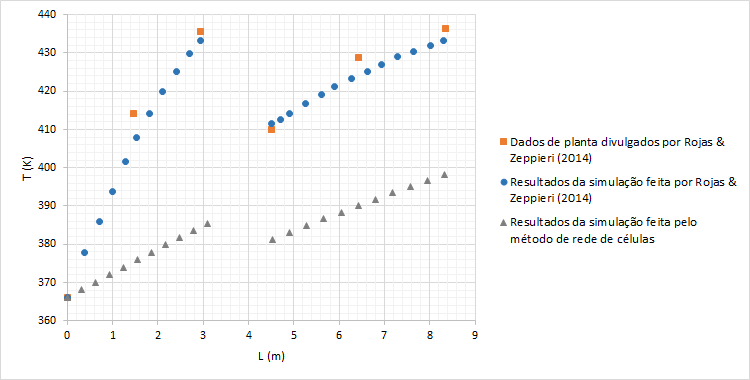
\includegraphics[scale=0.4]{images/Chap4/perfilTvalidacao.png}
\caption{Perfil de temperatura dos leitos.}
\label{fig:perfilTvalidacao}
\end{figure}

Duas questões precisam ser destacadas da \autoref{fig:perfilTvalidacao}.
A primeira delas refere-se a exortermia dos leitos catalíticos: a modelagem aqui
desenvolvida apresenta exortemia inferior aos demais dados. Esse fato, quando
analisado isoladamente, induz ao pensamento de que ou a simulação por rede de
células não fora bem equacionada ou a abordagem é inadequada para o sistema
estudado.

A segunda questão refere-se ao resfriamento na região zona de \emph{quench}. O
dado de planta apresenta um resfriamento de \SI{25.7}{K} entre os leitos
catalíticos; a simulação de \citeonline{Rojas2014a} apresenta resfriamento de
\SI{21,6}{K} para a região; e o valor encontrado no presente trabalho foi de
\SI{4,1}{K}. Essa situação torna-se mais enigmática ao se constatar que o
balanço de energia proposto por \citeonline{Rojas2014a} para a região de \emph{quench}
é ainda mais simplificado que o proposto neste estudo.

Uma análise do valor de LHSV (\emph{Liquid Hourly Space Velocity}) foi feita
na tentativa de trazer um esclarecimento às discrepâncias encontradas. O
parâmetro LHSV pode ser definido como: 
\begin{equation}
\textrm{LHSV} = F_{vol}^L/{V_{R}}
\label{eq:LHSV}
\end{equation}
onde $F_{v}^L$ é a vazão volumétrica em \si{m^3/h} de líquido e $V_{R}$ é o
volume total do reator (somados os dois leitos).

\nomenclature{$F_v$}{Vazão volumétrica \nomunit{m^3/h}}
\nomenclature[S]{$v$}{Referente ao volume}
\nomenclature{$V$}{Volume \nomunit{m^3}}
\nomenclature{$V_R$}{Volume total do reator \nomunit{m^3}}

A \autoref{tab:comparacaoLHSV} mostra alguns valores encontrados na literatura
para LHSV, incluindo o trabalho de \citeonline{Rojas2014a}.

\begin{table}[!htb]
\begin{center}
\caption{Comparação entre valores de LHSV calculados com base em dados publicados na literatura.}
\label{tab:comparacaoLHSV}
\small
\begin{tabular}{lccc}
{Autor} & {$F_v^L$ (\si{m^3/h})} & {$V_R$ (\si{m^3})} &
{LHSV (\si{1/h})}
\\
\hline
{\citeonline{Arpornwichanop2008}} & 69 & 60 & 1.14 \\
{\citeonline{Mederos2007}} & 165 & 62 & 2.66 \\
{\citeonline{Rojas2014a}} & 347 & 18 & 19.76 \\
\bottomrule
\end{tabular}
\end{center}
\end{table}

Comparativamente fica claro que o valor de LHSV do trabalho de
\citeonline{Rojas2014a} está uma ordem de grandeza acima dos valores
comumente empregados nos projetos de reatores TBR.

?? Comentar algo do tipo:
Infelizmente, até o presente momento, não foi possível contactar os
autores do trabalho de \citeonline{Rojas2014a} para a verificação
dos valores publicados.
??
Sendo assim, foi necessário ajustar o valor da vazão de alimentação de gasolina
de pirólise para que os dados apresentassem coerência. O critério utilizado foi
o grau de resfriamento que ocorre na região de \emph{quench}. De maneira mais
direta, a vazão ?? de \emph{quench} ?? foi modificata até que a diferença de temperatura entre a saída
do primeiro leito e entrada do segundo fossem semelhantes aos dados de planta e,
também, aos demais dados calculados por \citeonline{Rojas2014a}.

Após várias tentativas, o valor de $F_{w,1}$ foi alterado para \SI{2,079e4}
{kg/h}. Com essa nova vazão, tanto o resfriamento da região de \emph{quench}
quando a exotermia dos leitos tornaram-se aderentes aos dados de planta e de
literatura, como está mostrado na \autoref{sec:estadoestacionario}.

A \autoref{tab:comparacaoLHSV2} repete os valores da
\autoref{tab:comparacaoLHSV}, mas agora com a inclusão do valor de LHSV
após o ajuste da vazão de carga do reator.

\begin{table}[!htb]
\begin{center}
\caption{Comparação entre LHSV}
\label{tab:comparacaoLHSV2}
\small
\begin{tabular}{lccc}
{Autor} & {$F_v^L$ (\si{m^3/h})} & {$V_R$ (\si{m^3})} &
{LHSV (\si{1/h})}
\\
\hline
{\citeonline{Arpornwichanop2008}} & 69 & 60 & 1.14 \\
{\citeonline{Mederos2007}} & 165 & 62 & 2.66 \\
{\citeonline{Rojas2014a}} & 347 & 18 & 19.76 \\
{Dados ajustados} & 76 & 18 & 4.34 \\
\bottomrule
\end{tabular}
\end{center}
\end{table}

\subsection{Determinação do Valor de $N_{Disc}$} \label{sec:determinacaoNDisc}

Nesta seção será apresentada a maneira como foi escolhido o valor ideal de
$N_{Disc}$. O valor escolhido foi utilizado em todas as simulações doravante
apresentadas.

A maneira mais simples (e talvez a mais adequada) de se determinar o número de
células é simular o reator com diferentes valores de $N_{Disc}$ e, então,
verificar os resultados de algumas variáveis chave. Duas variáveis
foram escolhidas: temperatura e fração molar global de hidrogênio.

A \autoref{fig:NDiscT} mostra o perfil de temperatura do leito superior, para
diferentes valores de $N_{Disc}$. Percebe-se que, entre $N_{Disc} = 4$ e
$N_{Disc} = 8$ ainda há alguma diferença no comportamento do perfil de
temperatura. Contudo, é imperceptível a diferença entre os perfis resultantes de
$N_{Disc} = 8$ e $N_{Disc} = 16$. 

\begin{figure}[htb] \centering
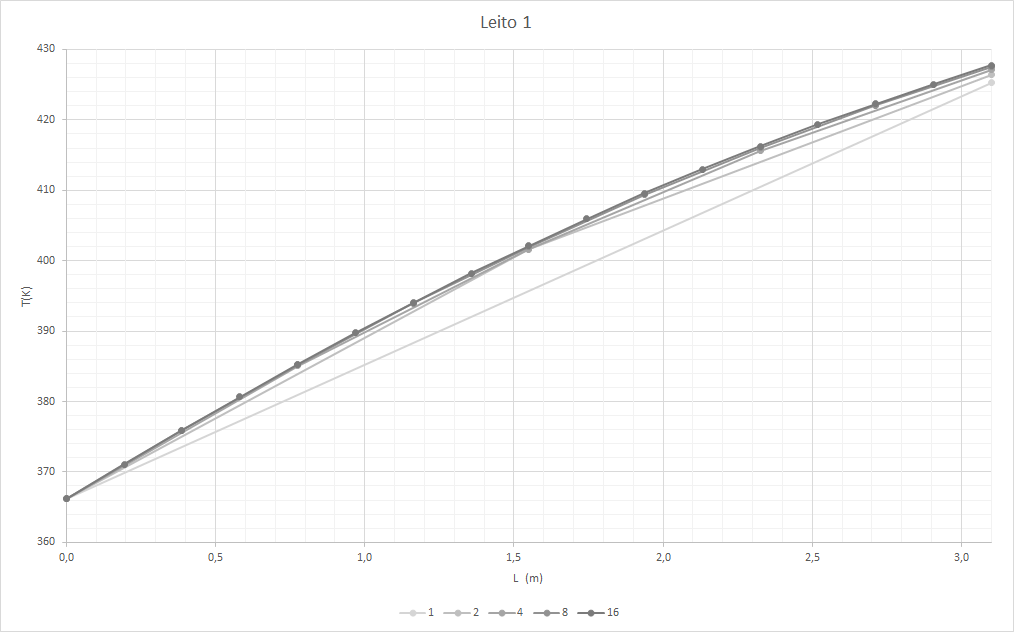
\includegraphics[scale=0.4]{images/Chap4/NDiscT.png}
\caption{Avaliação de NDisc pelo perfil de temperatura.}
\label{fig:NDiscT}
\end{figure}

Observando o perfil da fração molar global de hidrogênio de diferentes valores
de $N_{Disc}$ (também para o leito superior), é ainda menos relevante a
diferença entre $N_{Disc} = 4$ e $N_{Disc} = 8$, como mostra a
\autoref{fig:NDiscz}.

\begin{figure}[htb]
\centering 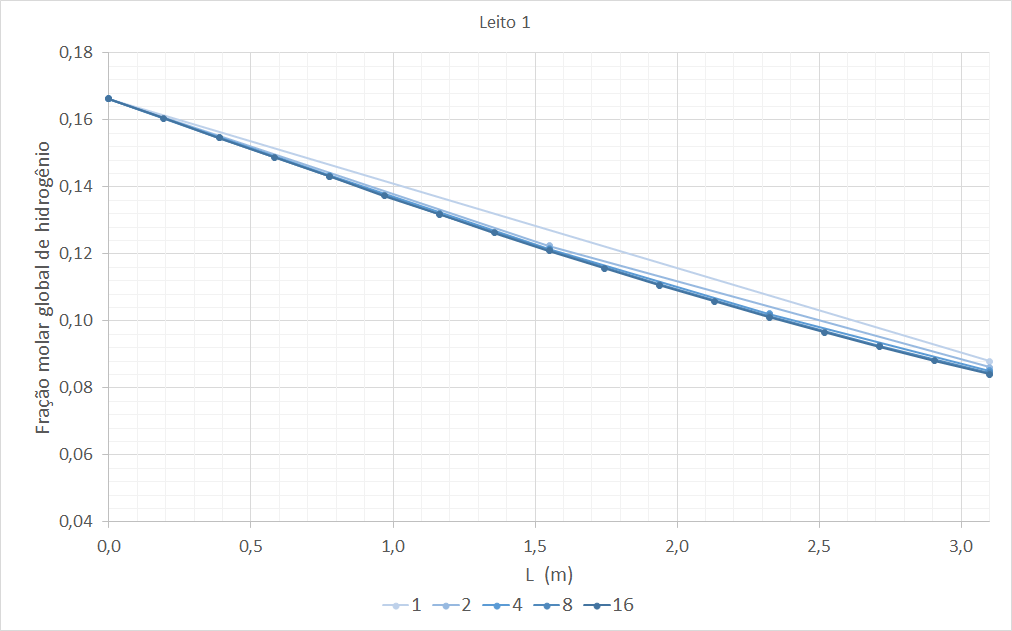
\includegraphics[scale=0.4]{images/Chap4/NDiscz.png}
\caption{Avaliação de NDisc pela fração molar total de hidrogênio.}
\label{fig:NDiscz}
\end{figure}

Assim, discretizar cada leito catalítico em $8$ células pareceria uma escolha
razoável e suficiente para o objetivo deste trabalho. Entretanto, para
garantir a representação dos leitos como contínuos, foi utilizado um valor um
pouco maior, $N_{Disc} = 10$.
Esta escolha faz com que o modelo apresente um total de ?? variáveis quando
computadas todas as variáveis intermediárias relacionadas com a hidrodinâmica.
E um todal de ?? variáveis quando as variáveis relacionadas com a hidrodinâmica
são ignoradas e a perda de carga é desprezada.

\subsection{Avaliação da Perda de Carga} \label{sec:avaliacaoperdadecarga}

A equação da perda de carga quando implementada no modelo do reator causou
alguns problemas de convergência. Assim, optou-se primeiramente por avaliar a
importância da perda de carga, e se ela alteraria muito o perfil de pressão a
ponto de impactar no cálculo das propriedades das fases e do ELV.

Foi feita, portanto, uma simulação inicial que estimou a perda de carga, mas sem
alterar o perfil de pressão (pressão constante ao longo do reator). A perda de
carga estimada para os leitos está na \autoref{tab:perdadecarga}. Por esses
valores, percebe-se que a pressão ao longo dos leitos permanece praticamente
inalterada. Sendo assim, o reator foi simulado desprezando-se a perda de carga.

\begin{table}[!htb]
\begin{center}
\caption{Avaliação da perda de carga dos leitos.}
\label{tab:perdadecarga}
\small
\begin{tabular}{lccc}
{} & {$\Delta P/L$ (\si{atm/m})} & {Pressão de entrada (\si{atm})} & {Pressão de saída
(\si{atm})}
\\
\hline
{Leito 1} & \num{3.4e-3} & 49.64 & 49.63 \\
{Leito 2} & \num{3.7e-3} & 49.63 & 49.61 \\
\bottomrule
\end{tabular}
\end{center}
\end{table}

Um valor tão baixo assim de perda de carga não é o comumente encontrado na
indústria. Porém, a equação utilizada por \citeonline{Rojas2014a} e aqui neste
trabalho pode não ser a mais adequada, já que houve uma alteração da vazão de
carga do reator. Está mostrado na \autoref{sec:estadoestacionario} que o regime
de escoamento do reator se altera de regime de bolha (alta interação),
considerado por \citeonline{Rojas2014a}, para regime de escoamento gotejante
(baixa interação). Assim sendo, a equação para avaliação da perda de carga no
reator deveria ter sido outra mais adequada às características do sistema.

\section{Estado Estacionário} \label{sec:estadoestacionario}

\subsection{Perfil de Temperatura} \label{sec:perfildetemperatura}

A \autoref{fig:perfilT} mostra o perfil de temperatura dos leitos
calculado por este trabalho, além daquele calculado por \citeonline{Rojas2014a}
e pelos dados de planta por eles publicados.  

\begin{figure}[htb]
\centering 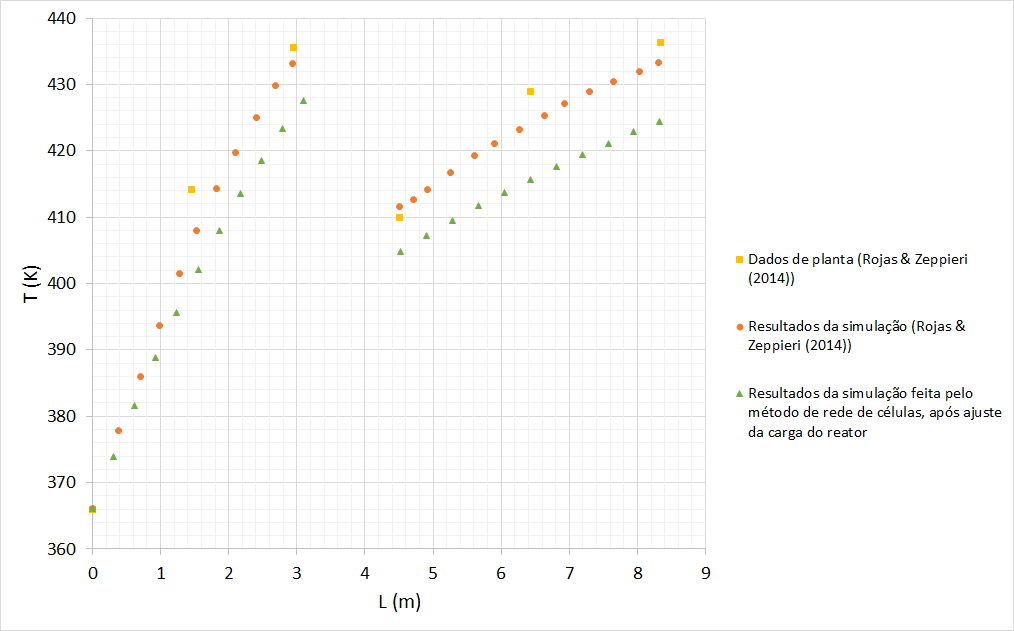
\includegraphics[width=0.8\textwidth]{images/Chap4/perfilT.png}
\caption{Perfil de temperatura dos leitos.}
\label{fig:perfilT}
\end{figure}

A diminuição drástica do valor da vazão de alimentação está refletida na alteração
do perfil de temperatura primeiramente encontrado
(\autoref{fig:perfilTvalidacao}). Sendo o perfil de temperatura obtido neste
trabalho semelhante tanto aos dados de planta quando aos valores calculados por
\citeonline{Rojas2014a}, é possível apresentar os demais resultados e efetuar
mais comparações.


\subsection{Composição da Corrente Efluente do Reator}
\label{composicaodacorrenteefluentedoreator}

\citeonline{Rojas2014a} divulgaram a composição do efluente do reator agrupando
alguns compostos. Assim sendo, foi implementado o mesmo agrupamento para fins de
comparação, como mostra a \autoref{tab:composicaodoefluente}. Pela comparação
entre os dados composicionais do efluente do reator, corrobora-se a opção de se
alterar a vazão de alimentação.

\begin{table}[!htb]
\begin{center}
\caption{Composição do Efluente do Reator em Fração Molar}
\label{tab:composicaodoefluente}
\small
\begin{tabular}{lccc}
{Compostos} & {Dados de Planta} & {\citeonline{Rojas2014a}} & {Este Trabalho}
\\
\hline
{Hidrogênio} & 0.06 & 0.05 & 0.04 \\
{C1-C4 não reativos} & 0.05 & 0.04 & 0.04 \\
{C6-C9 não reativos} & 0.06 & 0.07 & 0.06 \\
{Benzeno-Tolueno-Xileno} & 0.48 & 0.47 & 0.48 \\
{Dienos C5-C6} & 0.00 & 0.00 & 0.00 \\
{Olefinas C5-C6} & 0.14 & 0.15 & 0.14 \\
{Parafinas C5-C6} & 0.10 & 0.12 & 0.14 \\
{Estirenos} & 0.00 & 0.00 & 0.00 \\
{Aromáticos reativos} & 0.06 & 0.07 & 0.07 \\
{Diciclodienos} & 0.00 & 0.00 & 0.00 \\
{Diciclodienos hidrogenados} & 0.03 & 0.03 & 0.03 \\
\bottomrule
\end{tabular}
\end{center}
\end{table}

\subsection{ELV} \label{elv}

Como está mencionado no \autoref{chap:moddesenvolvidos}, a fração de vapor
em cada célula $z$ é determinada por um cálculo de \emph{flash}, implementado no
modelo \code{streamTP}, detalhado no \autoref{chap:streamTP}. A
\autoref{fig:perfilfracaovaporizada} mostra o perfil da fração de vapor (base
molar) ao longo do leito catalítico.

\begin{figure}[htb]
\centering 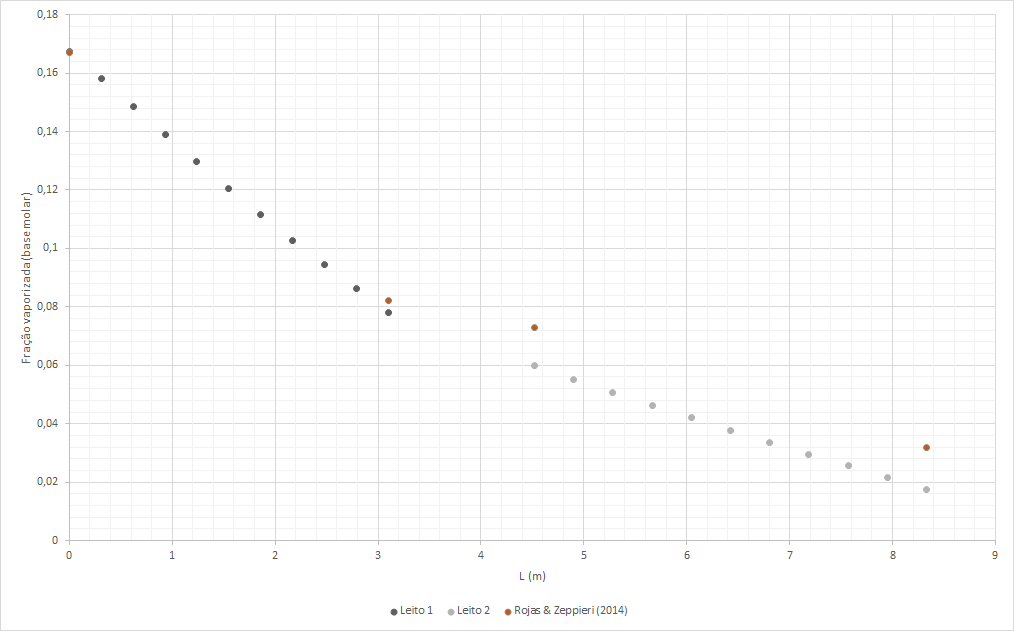
\includegraphics[scale=0.4]{images/Chap4/perfilfracaovaporizada.png}
\caption{Perfil de fração vaporizada}
\label{fig:perfilfracaovaporizada}
\end{figure}

É possível perceber pela \autoref{fig:perfilfracaovaporizada} que a fração
vaporizada na entrada do primeiro leito calculada neste trabalho é muito próxima
daquela calculada por \citeonline{Rojas2014a}. Já para o segundo leito, há uma
diferença próxima a 20\% entre os dois conjuntos de resultados.

Duas questões entre o presente trabalho e o publicado por
\citeonline{Rojas2014a} podem justificar essa diferença.

A primeira delas é a questão da perda de carga. Neste trabalho, como explicado
na \autoref{sec:avaliacaoperdadecarga}, a perda de carga fora desprezada. Visto
que \citeonline{Rojas2014a} não publicaram o valor da perda de carga encontrada nos
leitos catalíticos, não é possível avaliar se há ou não uma influência da perda
de carga na fração vaporizada.

Há ainda outra diferença: o parâmetro de interação binaria $\delta_{ij}$ foi
calculada por \citeonline{Rojas2014a} utilizando a base de dados do software
comercial PRO/II 9.0. Ainda, a regra de mistura por eles apontada como a de melhor resultado (e,
entende-se como sendo a que foi utilizada para gerar os resultados publicados)
foi a de PA-RESimSci (SimSci-Esscor. PRO/II 9.0 Component and Thermophysical
Properties Reference Manual (2010)).

\subsection{Comportamento do Hidrogênio} \label{comportamentodohidrogenio}

Uma das premissas adotadas aqui, e que é oriunda do trabalho de
\citeonline{Rojas2014a}, é que a concentração de hidrogênio na
fase líquida é aproximadamente constante ao longo do reator. Por essa razão,
outra premissa também foi considerada, a de que as reações podem ser
consideradas como de pseudo-primeira ordem, desprezando a concentração de
hidrogênio.

A \autoref{fig:perfilfracaoh2liquido} confirma a premissa adotada, mostrando que
a fração molar de hidrogênio em fase líquida ao longo do reator não só é
praticamente constante, como também aumenta ao longo do reator. A
\autoref{fig:perfilfracaoh2liquido} também está em acordo com o
comportamento do hidrogênio de ser tanto mais solúvel em hidrocarbonetos
líquidos quanto maior for a temperatura, como mostra melhor a
\autoref{fig:perfilfracaoh2temperatura}.
?? como foi construida esta última figura, detalhar no texto se é apenas
uma reorganização da anterior com outras variáveis. Se sim, para qual leito ??

\begin{figure}[htb]
\centering 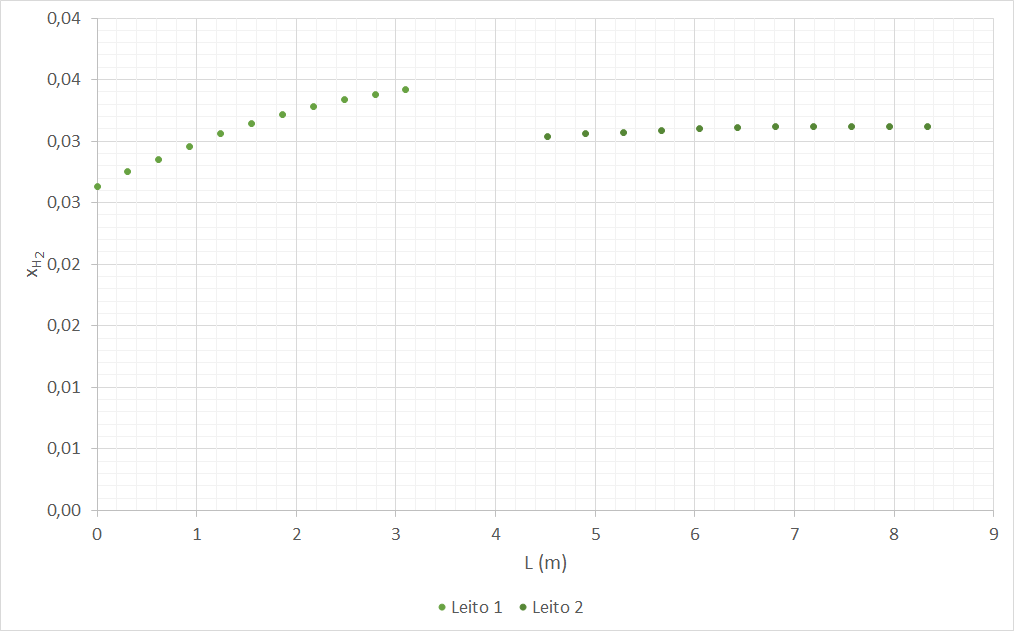
\includegraphics[scale=0.4]{images/Chap4/perfilfracaoh2liquido.png}
\caption{Perfil de fração ?? molar ?? de hidrogênio em fase líquida.}
\label{fig:perfilfracaoh2liquido}
\end{figure}

\begin{figure}[htb]
\centering
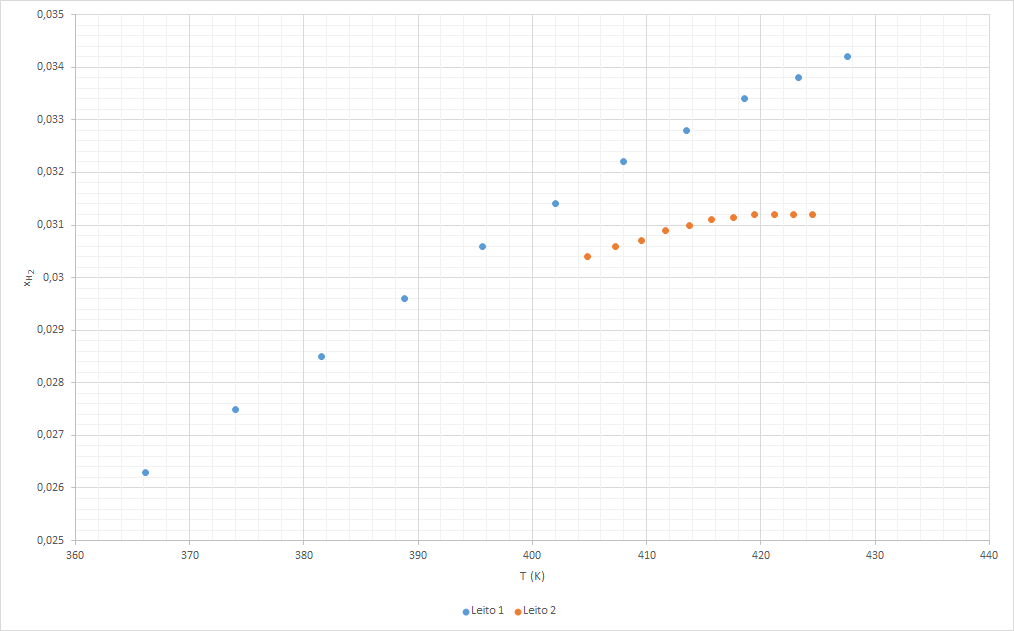
\includegraphics[scale=0.4]{images/Chap4/perfilfracaoh2temperatura.png}
\caption{Fração ?? molar ?? de hidrogênio em fase líquida \emph{vs.} da temperatura.}
\label{fig:perfilfracaoh2temperatura}
\end{figure}

A \autoref{fig:perfilfracaoh2gas} mostra o comportamento da
fração molar de hidrogênio na fase gasosa. Por ser consumido conforme as reações
avançam ao longo dos leitos catalíticos, o hidrogênio tende a diminuir de
concentração na fase gasosa ao longo do reator, como já era esperado.

\begin{figure}[htb]
\centering
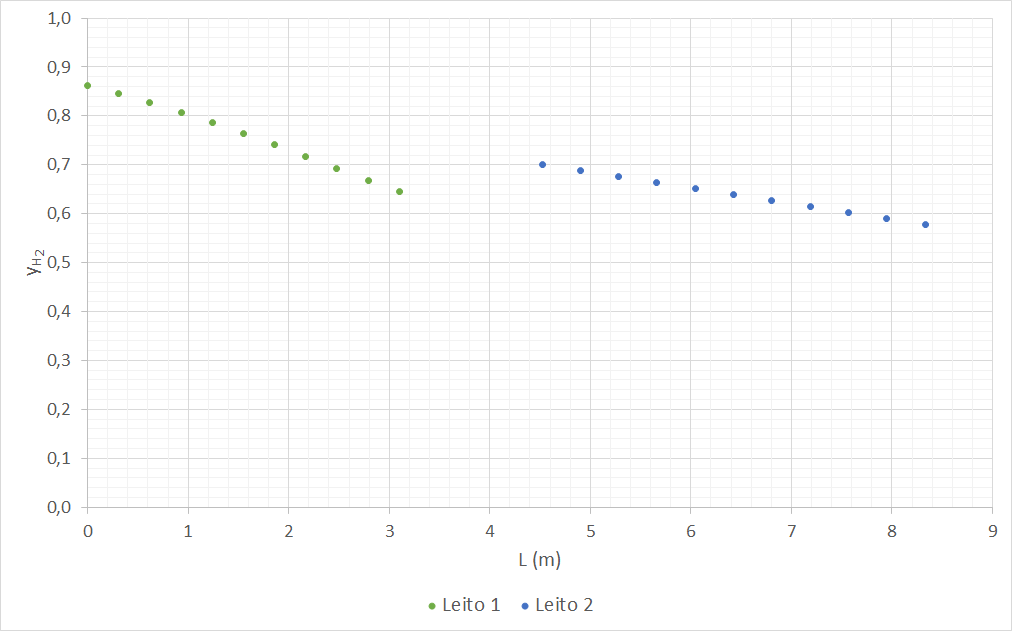
\includegraphics[scale=0.4]{images/Chap4/perfilfracaoh2gas.png}
\caption{Perfil de fração de hidrogênio em fase gasosa}
\label{fig:perfilfracaoh2gas}
\end{figure}

\subsection{Propriedades Termodinâmicas} \label{propriedadestermodinâmicas}

A \autoref{tab:propriedadestermodinamicas} apresenta os valores de algumas
propriedades termodinâmicas calculadas neste trabalho.

\begin{table}[!htb]
\begin{center}
\caption{Propriedades Termodinâmicas}
\label{tab:propriedadestermodinamicas}
\small
\begin{tabular}{lcccc}
{Propriedade} & {Entrada Leito 1} & {Saída Leito 1} & {Entrada Leito 2} &
{Saída Leito 2}
\\
\hline
{$MW^{L}$ (\si{kg/kmol})} & 82.5 & 81.6 & 81.6 & 81.2 \\
{$MW^{G}$ (\si{kg/kmol})} & 7.0 & 18.4 & 13.6 & 18.8 \\
{$\rho^{L}$(\si{kg/m^3})} & 728.7 & 639.9 & 668.9 & 635.3 \\
{$\rho^{G}$ (\si{kg/m^3})} & 11.4 & 26.4 & 20.3 & 27.2 \\
\bottomrule
\end{tabular}
\end{center}
\end{table}

Conforme já esperado, o resultado da simulação mostra que a densidade do líquido
diminui ao longo do primeiro leito catalítico (conforme há aumento de
temperatura), aumenta na região de \emph{quench} (devido à injeção de líquido
frio), e volta a diminuir ao longo do segundo leito. A densidade da fase gasosa
tem o comportamento inverso, já que conforme a temperatura aumenta, para uma
mesma pressão, a densidade de um gás tende a aumentar.
?? esta última explicação não está coerente ??

A massa molar do líquido tende a permanecer constante ao longo de todo o
reator, mostrando que o aumento da concentração de hidrogênio não é relevante
para alterar significativamente essa propriedade.

Mudança mais relevante sofre a massa molar da fase gasosa, que aumenta ao
longo do primeiro e segundo leitos, diminuindo na zona de \emph{quench}. Esse
comportamento é reflexo tanto da diminuição da concentração de hidrogênio na
fase gasosa, que tende a se diluir mais facilmente em fase líquida conforme a
temperatura aumenta, quanto da evaporação de compostos leves conforme o leito
catalítico aquece.

Os resultados das propriedades termodinâmicas parecem mais aderentes com
aqueles divulgados por \citeonline{Rojas2014a}. A diferença pode ser explicada
tanto por conta do pacote termodinâmico utilizado quanto pelo perfil de
temperatura resultante da simulação por eles realizada.

\subsection{Propriedades Hidrodinâmicas} \label{propriedadeshidrodinâmicas}

A \autoref{tab:propriedadeshidrodinamicas} mostra o resultado de algumas
propriedades hidrodinâmicas e números adimencionais utilizados nos cálculos de
transferência de massa e perda de carga.

\begin{table}[!htb]
\begin{center}
\caption{Propriedades Hidrodinâmicas}
\label{tab:propriedadeshidrodinamicas}
\small
\begin{tabular}{lcccc}
{Propriedade} & {Entrada Leito 1} & {Saída Leito 1} & {Entrada Leito 2} &
{Saída Leito 2}
\\
\hline
{$u^{L}$ (\si{m/s})} & \num{3.2e-3} & \num{3,6e-3} & \num{4,7e-3} & \num{4,9e-3} \\
{$u^{G}$ (\si{m/s})} & \num{3,3e-3} & \num{1,7e-3} & \num{1,5E-3} & \num{0,5E-3} \\
{$\mu^{L}$(\si{cP})} & \num{0,128} & \num{0,103} & \num{0,130} & \num{0,121} \\
{$\mu^{G}$ (\si{cP})} & \num{0,012} & \num{0,013} & \num{0,012} & \num{0,013} \\
{$Re^{L}$} & \num{54,4} & \num{67,6} & \num{72,1} & \num{78,0} \\
{$Re^{G}$} & \num{10,6} & \num{10,1} & \num{7,6} & \num{3,0} \\
{$Ga^{L}$} & \num{8,6e6} & \num{10,4e6} & \num{7,0e6} & \num{7,4e6} \\
{$We^{L}$} & \num{1,5e-3} & \num{2,8e-3} & \num{4,1e-3} & \num{5,2e-3} \\
{$X^{G}$} & \num{7,8} & \num{2,3} & \num{1,8} & \num{0,5} \\
{$Pe^{L}$} & \num{428} & \num{443} & \num{600} & \num{609} \\
\bottomrule
\end{tabular}
\end{center}
\end{table}

É preciso informar aqui que os valores de $\mu^L$ e $\mu^G$ apresentados na
\autoref{tab:propriedadeshidrodinamicas} foram calculadas por rotinas internas
do simulador iiSE; os demais parâmetros foram calculados por equações
apresentadas na \autoref{chap:moddesenvolvidos}. Ademais, o comportamento da
viscosidade das fases foi como o esperado, ou seja, a viscosidade da fase
líquida diminui com o aumento da temperatura, e a viscosidade da fase gasosa
aumenta com o mesmo aumento (considerando que a pressão ao longo do reator é
constante).

Um resultado que chama a atenção na \autoref{tab:propriedadeshidrodinamicas}
refere-se à velocidade de escoamento das fases e, consequentemente, ao número de
Reynolds delas. A velocidade da fase líquida divulgada por
\citeonline{Rojas2014a}, por exemplo, esteve entre \SI{1,2e-2}{m/s} e
\SI{1,5e-2}{m/s}, o que é cerca de cinco vezes maior do que os valores
encontrados neste trabalho. Aqui, portanto, fica clara a divergência da vazão de
carga do reator utilizada neste trabalho e no trabalho original.

Os números de $Ga^L$ e $We^L$ foram usados para o cálculo de $\eta_{CE}$ e
$\epsilon^{L}$, respectivamente. Esses parâmetros estão apresentados nas seções
a seguir.

\subsubsection{Retenção Total de Líquido $\epsilon^{L}$}
\label{retencaototaldeliquido}

A \autoref{fig:perfilretencaoliquido} mostra o perfil da retenção de líquido
total $\epsilon^{L}$ ao longo dos leitos. Considerando que, ao longo do leito, a fração vaporizada diminui
(\autoref{tab:comparacaoLHSV2}), é coerente que a retenção de líquido aumente.
Do primeiro leito para o segundo leito há um aumento da retenção de líquido, que
é fruto do aumento da vazão de líquido dentro do reator causado pela injeção da
corrente líquida de \emph{quench}.

\begin{figure}[htb]
\centering
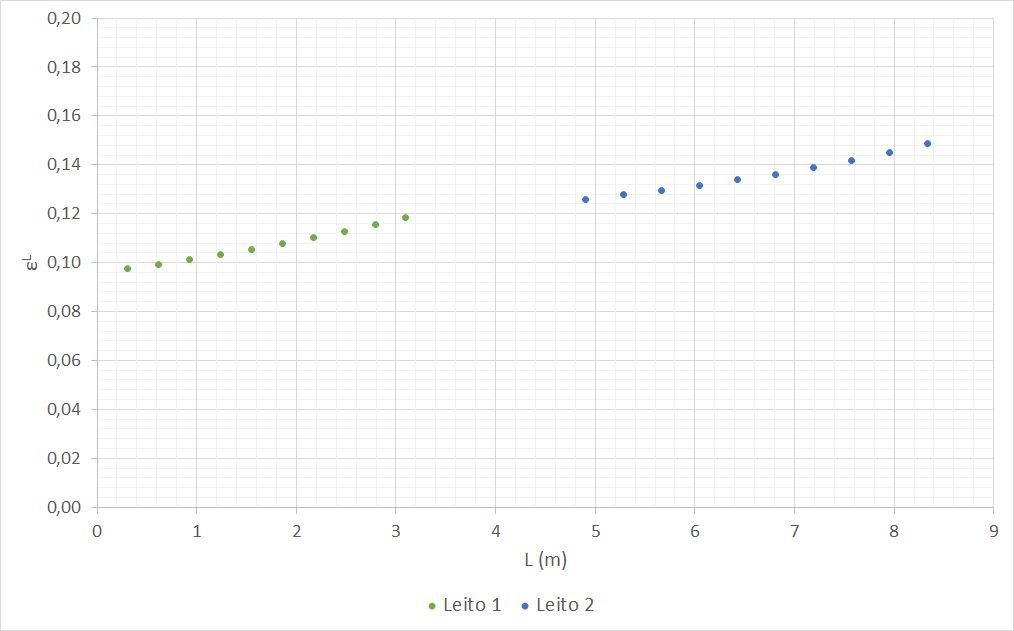
\includegraphics[scale=0.4]{images/Chap4/perfilretencaoliquido.png}
\caption{Perfil de $\epsilon^{L}$}
\label{fig:perfilretencaoliquido}
\end{figure}

Como já explicado no \autoref{chap:moddesenvolvidos}, a variável $\epsilon^{L}$
possui como dimensão o valor de $N_{Disc}$.

Os valores $\epsilon^{L}$ encontrados por \citeonline{Rojas2014a} foram de
0,14 e 0,17 para a entrada do Leito 1 e saída do Leito 2,
respectivamente. A diferença entre os resultados pode ser explicada pela
incerteza quanto à vazão de carga no reator, que neste trabalho precisou ser
modificada por motivos já explicados. Contudo, a diferença não é tão
significativa assim, sendo ambos os trabalhos aderentes aos resultados de
literatura.

\subsubsection{Eficiência de Molhamento} \label{eficienciademolhamento}

A eficiência de molhamento $\eta_{CE}$ para o primeiro e o segundo leitos
catalíticos do reator aqui estudado foi estimada em \SI{0,72} e \SI{0,75},
respectivamente. Em seu trabalho, \citeonline{Rojas2014a} encontraram valores
maiores do que \SI{1,0} para o parâmetro $\eta_{CE}$.

Este é mais um caso onde a incerteza quanto à vazão de carga do reator
impossibilita uma análise comparativa mais acurada. De qualquer forma, vale a
observação de que, por possuir uma vazão de líquido maior devido a injeção da
corrente de \emph{quench}, o segundo leito do reator apresenta eficiêcia de
molhamento maior do que o primeiro, como já era esperado.

\subsubsection{Escoamento - Classificação} \label{escoamentoclassificacao}

Segundo \citeonline{Sie1998}, o regime de escoamento gotejante é definido
principalmente pelas velocidades superficiais das fases gás e líquida. Neste
trabalho há uma figura em que, de acordo com as velocidades superficiais das
fases, é possível verificar o tipo de escoamento no qual o reator opera. Segundo
essa figura, o reator estudado neste trabalho enquadra-se como um reator de
leito gotejante.

\citeonline{Saroha1996} publicaram um mapa mais elaborado que classifica o
escoamento dos reatores trifásicos de leito fixo. De acordo com esse mapa, os
valores encontrados na presente simulação colocam o reator objeto de estudo na
região de escoamento tipo leito gotejante.

Assim, o tipo de escomento encontrado aqui para o reator é contrário à premissa
adotada de escoamento tipo bolha. É preciso lembrar que este trabalho
preocupou-se em manter ao máximo as premissas e valores publicados por
\citeonline{Rojas2014a}. Contudo, a premissa adotada para o tipo de escoamento
(borbulhamento), que influencia na escolha das equações hidrodinâmicas, deveria
ser revista e outras equações hidrodinâmicas deveriam ter sido utilizadas no
lugar das atuais.

\subsection{Transferência de Massa - Interface Líquido-Sólido}
\label{transferênciademassainterfaceliquidosolido}

Como assumido nas premissas deste trabalho, a transferência de massa entre as
fases gasosa e líquida foi desprezada, ficando então a composição \emph{bulk}
destas fases definida pelo ELV.

Já a composição dos reagentes e produtos na superfície do catalisador ($C^S$)
foi considerada distinta da composição \emph{bulk} da fase líquida $C^L$. A
\autoref{tab:concentraçõesparaoleito1} mostra as concentrações dos compostos na
fase líquida (\emph{bulk}) e na superfície do catalisador para a entrada e a
saída do Leito 1. De acordo com os resultados, fica evidente que a diferença dos
valores de $C^S$ e $C^L$ para cada um dos compostos é mínima.

Assim, a taxa da reação poderia muito bem ser calculada com a composição
\emph{bulk} da fase líquida $C^L$, desprezando-se a transferência de massa na
interface líquido-sólido.

\begin{table}[!htb]
\begin{center}
\caption{Concentrações $C^L_{i}$ e $C^S_{i}$ para o Leito 1}
\label{tab:concentraçõesparaoleito1}
\small
\begin{tabular}{lcccc}
{Composto} & {$C^{L}_{1}$} & {$C^{S}_{1}$} & {$C^{L}_{11}$} & {$C^{S}_{11}$}
\\
\hline
{Hidrogênio} & 0.2397 & 0.2367 & 0.2656 & 0.2644 \\
{Metano} & 0.1002 & 0.1002 & 0.1304 & 0.1304 \\
{Etano} & 0.0210 & 0.0210 & 0.0208 & 0.0208 \\
{n-Propano} & 0.0511 & 0.0511 & 0.0468 & 0.0468 \\
{n-Butano} & 0.0352 & 0.0352 & 0.0312 & 0.0312 \\
{n-Pentano} & 0.5327 & 0.5328 & 0.5070 & 0.5073 \\
{trans-2-Penteno} & 0.5512 & 0.5519 & 0.5876 & 0.5879 \\
{trans-1.3-Pentadieno} & 0.2455 & 0.2447 & 0.0739 & 0.0734 \\
{Ciclopentano} & 0.1557 & 0.1559 & 0.1911 & 0.1914 \\
{Ciclopenteno} & 0.2539 & 0.2554 & 0.3054 & 0.3053 \\
{Metil-1.3-Ciclopentadieno} & 0.1611 & 0.0210 & 0.0208 & 0.0208 \\
{n-Hexano} & 0.2757 & 0.2757 & 0.2424 & 0.2424 \\
{Metilciclopentano} & 0.1383 & 0.1383 & 0.1370 & 0.1371 \\
{Metilciclopenteno} & 0.1866 & 0.1871 & 0.2428 & 0.2430 \\
{1.3-Ciclopentadieno} & 0.1695 & 0.1680 & 0.0128 & 0.0126 \\
{Benzeno} & 2.6803 & 2.6803 & 2.3579 & 2.3579 \\
{n-Heptano} & 0.2029 & 0.2029 & 0.1786 & 0.1786 \\
{Tolueno} & 1.2642 & 1.2642 & 1.1141 & 1.1141 \\
{n-Octano} & 0.0825 & 0.0825 & 0.0727 & 0.0727 \\
{Etilbenzeno} & 0.2536 & 0.2546 & 0.3146 & 0.3148 \\
{Estireno} & 0.1207 & 0.1197 & 0.0156 & 0.0155 \\
{Xileno} & 0.3712 & 0.3712 & 0.3277 & 0.3277 \\
{n-Nonano} & 0.0376 & 0.0376 & 0.0332 & 0.0332 \\
{1-Metil-3-Etilbenzeno} & 0.1813 & 0.1816 & 0.2081 & 0.2083 \\
{Metilestireno} & 0.0813 & 0.0810 & 0.0239 & 0.0237 \\
{Dihidrodiciclopentadieno} & 0.2003 & 0.2014 & 0.2721 & 0.2724 \\
{Diciclopentadieno} & 0.1262 & 0.1251 & 0.0164 & 0.0161 \\
\bottomrule
\end{tabular}
\end{center}
\end{table}

\section{Respostas Dinâmicas} \label{sec:respostasdinamicas}

A simulação concebida neste trabalho nasceu preparada para estudos e avaliações
de respostas dinâmicas. Três avaliações de respostas dinâmicas foram feitas, a
saber:

\begin{enumerate}
  \item Resposta a um degrau na temperatura da carga, de \SI{366}{K} para
  \SI{300}{K};
  \item Resposta a um degrau na vazão da corrente de quench, de \SI{20790}{kg/h}
  para \SI{10790}{kg/h}; e
  \item Resposta a um degrau na vazão da corrente de quench, de \SI{20790}{kg/h}
  para \SI{30790}{kg/h}.
\end{enumerate}

As seções a seguir apresentam uma breve discussão para cada um dos casos
mencionados.

\subsection{Resposta a um degrau na temperatura da carga, de \SI{366}{K} para
\SI{300}{K}}
\label{sec:respostaaumdegrautemp}

Este primeiro caso reflete o comportamento do reator no caso da perda de
aquecimento da carga, seja por falta de utilidades (vapor para um trocador de
calor, por exemplo), seja por falha nos elementos primários de uma eventual
malha de controle.

Como consequência dessa perda de aquecimento da carga, o exotermia vista
em operação normal diminui drasticamente, sinal de que a conversão dos reagentes
passou a patamres inaceitáveis. O perfil de temperatura do Leito 1 do reator
após o degrau de temperatura na carga está mostrado na
\autoref{fig:FeedT300K}.

\begin{figure}[htb]
\centering
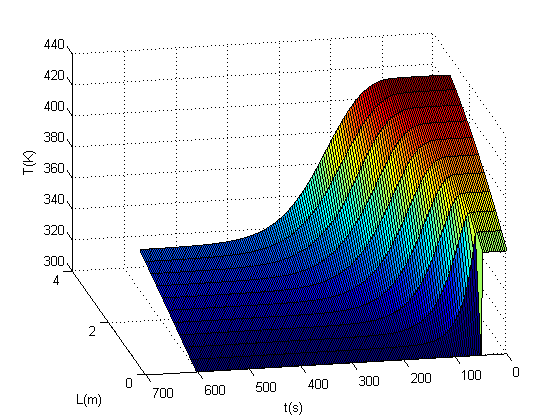
\includegraphics[scale=0.8]{images/Chap4/FeedT300K.png}
\caption{Resposta dinâmica a um degrau (queda) de temperatura na carga.}
\label{fig:FeedT300K}
\end{figure}

\subsection{Resposta a um degrau na vazão da corrente de \emph{quench}, de 20790
kg h para 10790 kg} \label{sec:respostaaumdegrauvazao1}

A perda de parte da vazão da corrente de \emph{quench} tem efeito imediato no
Leito 2 do reator, como mostra a \autoref{fig:QuenchF10790}.

\begin{figure}[htb]
\centering
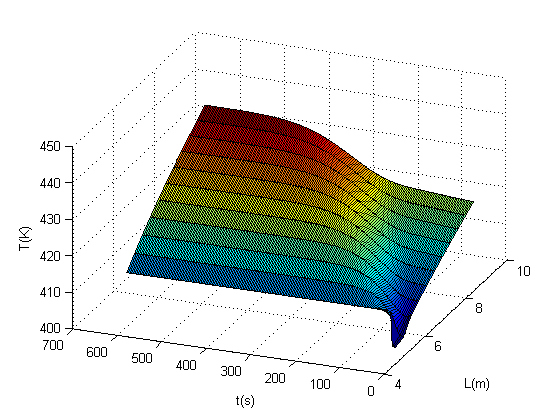
\includegraphics[scale=0.8]{images/Chap4/QuenchF10790.png}
\caption{Resposta dinâmica a um degrau (a menor) na vazão de \emph{quench}}
\label{fig:QuenchF10790}
\end{figure}

É importante notar aqui que a perda parcial da vazão de \emph{quench} poderia
levar algumas regiões do reator a temperaturas altas o suficiente para causar
disparos de temperatura. De qualquer forma, a exotermia observada significa
também maior conversão de olefinas que, para o objetivo desse processo (produzir
gasolina automotiva), tem efeito deletério quanto à octanagem.

\subsection{Resposta a um degrau na vazão da corrente de \emph{quench}, de 20790
kg h para 30790 kg} \label{sec:respostaaumdegrauvazao3}

Para a situação em que a vazão da corrente de \emph{quench} aumenta, quer seja
por problema de instrumentação ou equipameto, quer seja por erro humano, o Leito
2 é esfriado como mostra a Figura \autoref{fig:QuenchF30790}.

\begin{figure}[htb]
\centering
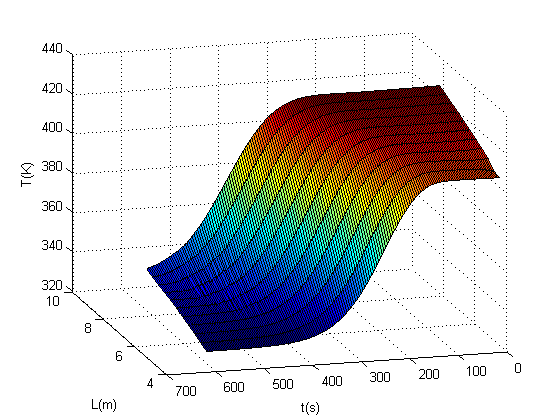
\includegraphics[scale=0.8]{images/Chap4/QuenchF30790.png}
\caption{Resposta dinâmica a um degrau (a maior) na vazão de \emph{quench}.}
\label{fig:QuenchF30790}
\end{figure}

Um problema neste caso é a queda na conversão dos compostos diolefínicos, o
que conferiria uma característica instável à gasolina automotiva.










%
% 
%
\chapter{Conclusões e Sugestões} \label{chap:conclusoes}
% 
% Como se sabe, a operação de colunas de destilação vem sendo estudada há muitos anos.
% Sabe-se também, que este
% equipamento é um dos mais importantes das indústrias químicas, petroquímicas e de alimentos. Sua
% importância não se resume só a sua função e operação, mas também devido ao fato de que
% colunas de destilação são responsáveis por grande parte do gasto de energia em uma
% indústria. Sendo assim, o desenvolvimento de modelos para estes equipamentos é uma tarefa
% relevante, tanto para projeto quanto para simulações de operação e otimização das
% unidades existentes.

Modelos matemáticos de colunas de destilação podem ser classificados de acordo com o seu
grau de detalhamento: se possuem predição da composição, temperatura e vazões para cada prato,
os chamados modelos rigorosos, ou se são compostos por uma descrição global da coluna
utilizando um menor número de variáveis, baseados em algum tipo de interpolação, os modelos
reduzidos. Neste trabalho, foram apresentadas as diversas formas de
modelagem de sistemas de separação e concluiu-se que a escolha das considerações
simplificativas varia com a aplicação do modelo. Em estudos onde são necessárias simulações
repetitivas, como em otimizações, os modelos reduzidos podem ser os indicados.
Mas, em estudos de partidas e paradas de colunas de destilação é importante que o
comportamento dinâmico do sistema seja bem representado levando ao uso de
modelos rigorosos completos. 

Na linha da modelagem baseada no equilíbrio termodinâmico entre as fases líquida e vapor, foram
desenvolvidos todos os modelos necessários para a confecção de um modelo genérico de coluna
de destilação. Os modelos foram implementados no simulador dinâmico de processos EMSO
utilizando seu ambiente de modelagem e sua linguagem própria. Os modelos gerados neste estudo
fazem parte da biblioteca EML (EMSO Model Library). Esta biblioteca é distribuída no conceito
de \emph{software} livre, disponibilizando todos os modelos via internet e sem
custo.

Um exemplo de uma coluna de destilação reativa serviu como ilustração para a aplicação
dos modelos desenvolvidos neste trabalho em partidas de unidades de separação.
Ao contrário da modelagem encontrada na literatura para esse tipo de sistema, a condição de
equilíbrio termodinâmico entre as fases líquida e vapor foi considerada desde o início da
simulação sem causar problemas de inicialização e integração, conforme alguns autores relatam.
A partida de uma
coluna vazia e fria foi simulada de acordo com três das estratégias convencionais encontradas
na literatura. Como esperado, a partida realizada com refluxo total para a coluna apresentou um
tempo de transientes maior que as demais. Além disso, o modelo apresentado se mostrou muito
indicado para simulações de partida, uma vez que possíveis dificuldades para a determinação de
seus principais parâmetros não afetam a análise do tempo de operação dinâmica.

Outro exemplo foi utilizado para a validação do modelo desenvolvido. Trata-se de uma coluna
deisobutanizadora da PETROBRAS composta de 80 pratos que separa isobutano de
uma mistura de 13 componentes. Algumas pequenas adaptações foram realizadas nos modelos e os resultados obtidos
foram satisfatórios. Tanto a resposta estacionária quanto o comportamento dinâmico da
unidade foram comparados. O problema gerou um sistema de mais de 6300 equações. Um período de
8 dias de operação com várias perturbações na carga e no refluxo da coluna foi simulado em
cerca de 19 minutos de CPU. Conclui-se com isto que este modelo pode ser aplicado para os
mais diversos fins, desde simulações de procedimentos de parada e partidas de unidades, até
estimações, otimizações e treinamento de operação.

Como perspectivas de trabalhos futuros, algumas melhorias podem ser feitas nos modelos apresentados.
Para tornar o modelo de prato ainda mais genérico, pode ser adicionada uma corrente material extra
correspondente a uma retirada lateral. Isto permitiria a modelagem de colunas de destilação de petróleo
sem utilizar separadores de correntes entre os estágios da coluna.
A modelagem fiel do controle de pressão do topo da torre através do \textit{hot bypass} também é um assunto
interessante a ser estudado. Provavelmente esta implementação melhoraria a capacidade de predição do modelo
principalmente nas condições do topo da coluna.
Além disso, alguns assuntos importantes sobre a modelagem
de sistemas de separação podem ser estudados.
Sabe-se que na indústria, grande parte das colunas de destilação operam muito próximo
do seu limite superior de capacidade. Assim, a previsão do fenômeno de inundação da torre
e suas conseqüências na eficiência de separação se torna muito interessante.
Além de colunas de destilação de pratos, as colunas recheadas também são muito utilizadas.
A adaptação dos modelos apresentados nesta dissertação para a
representação deste tipo de colunas deverá ser a continuidade deste trabalho.

 
 
% Comandos para as referencias bibliográficas
\newdimen\bibindent
\setlength\bibindent{1.5em} % identaçao das referencias
{ % Um lineskip menor neste contexto de referencias
\baselineskip 4.3mm
% Edite o arquivo ppgeq.bib com as suas próprias referências 
\bibliography{ppgeq}
} 

% Inclusao dos Appendices 
\appendix
%
%
%
\chapter{Modelo escrito para correntes $\emph{F}$ com cálculo de
\textit{flash}}
\label{chap:streamTP}

\lstinputlisting[firstline=1, lastline=55, numbers=none, language=EMSO,
label=code:streamTP] {images/Ap1/streamTP.mso}


%
%
%
\chapter{Modelo de reator de leito fixo}
\label{chap:modeloleitofixo}

\lstinputlisting[firstline=1, lastline=258, numbers=none, language=EMSO,
label=code:modeloleitofixo] {images/Ap1/FBR_bifasic_model_Pygas.mso}


%
%
%
\chapter{Código principal para solução do reator em estado estacionário}
\label{chap:codigoestacionario}

\lstinputlisting[firstline=1, lastline=664, numbers=none, language=EMSO,
label=code:codigoestacionario] {images/Ap1/Reactor.mso}


\end{document}
